% Capitolul 6: Selecția modelului și managementul riscului
% Statistica piețelor financiare -- Program de licență, Academia de Studii Economice din București
% GENERAT de latex/build_chapter6.py -- modificați generatorul, nu acest fișier.

\newcommand{\coursename}{Statistica piețelor financiare}
\def\sfmlang{ro}
% Preambul comun SFM -- Statistica piețelor financiare / Statistics of Financial Markets (Beamer, 16:9)
% Același design ca MFM. Înainte de % Preambul comun SFM -- Statistica piețelor financiare / Statistics of Financial Markets (Beamer, 16:9)
% Același design ca MFM. Înainte de % Preambul comun SFM -- Statistica piețelor financiare / Statistics of Financial Markets (Beamer, 16:9)
% Același design ca MFM. Înainte de \input{../../latex/preamble} se definește
%   \newcommand{\coursename}{Statistics of Financial Markets}      (EN)
%   \newcommand{\coursename}{Statistica piețelor financiare}       (RO)  și  \def\sfmlang{ro}
% Fișierele .tex se află în EN/Courses, EN/Seminars, RO/Cursuri, RO/Seminarii (două niveluri sub rădăcină).
% Deck-urile sînt generate de latex/build_chapterN.py / build_seminarN.py (vezi latex/sfm_build.py).

\documentclass[9pt, aspectratio=169, t]{beamer}
\providecommand{\coursename}{Statistics of Financial Markets}

% Ensure content fits on slides
\setbeamersize{text margin left=8mm, text margin right=8mm}

%=============================================================================
% THEME AND STYLE CONFIGURATION
%=============================================================================
\usetheme{default}
% Using default theme for clean header/footer control

% Color Palette (matching Redispatch PDF)
\definecolor{MainBlue}{RGB}{26, 58, 110}
\definecolor{AccentBlue}{RGB}{26, 58, 110}
\definecolor{IDAred}{RGB}{205, 0, 0}
\definecolor{DarkGray}{RGB}{51, 51, 51}
\definecolor{MediumGray}{RGB}{128, 128, 128}
\definecolor{LightGray}{RGB}{248, 248, 248}
\definecolor{VeryLightGray}{RGB}{235, 235, 235}
\definecolor{KeynoteGray}{RGB}{218, 218, 218}
\definecolor{SectionGray}{RGB}{120, 120, 120}
\definecolor{FooterGray}{RGB}{100, 100, 100}
\definecolor{Crimson}{RGB}{220, 53, 69}
\definecolor{Forest}{RGB}{46, 125, 50}
\definecolor{Amber}{RGB}{181, 133, 63}
\definecolor{Orange}{RGB}{230, 126, 34}
\definecolor{Purple}{RGB}{142, 68, 173}

% Gradient background (exact Keynote 315° gradient: white to RGB 218,218,218)
\setbeamertemplate{background}{%
    \begin{tikzpicture}[remember picture, overlay]
        \shade[shading=axis, shading angle=315,
        top color=white, bottom color=KeynoteGray]
        (current page.south west) rectangle (current page.north east);
    \end{tikzpicture}%
}
% Fallback solid color for compatibility
\setbeamercolor{background canvas}{bg=}

\setbeamercolor{palette primary}{bg=MainBlue, fg=white}
\setbeamercolor{palette secondary}{bg=MainBlue!85, fg=white}
\setbeamercolor{palette tertiary}{bg=MainBlue!70, fg=white}
\setbeamercolor{structure}{fg=MainBlue}
\setbeamercolor{title}{fg=IDAred}
\setbeamercolor{frametitle}{fg=IDAred, bg=}
\setbeamercolor{block title}{bg=MainBlue, fg=white}
\setbeamercolor{block body}{bg=VeryLightGray, fg=DarkGray}
\setbeamercolor{block title alerted}{bg=Crimson, fg=white}
\setbeamercolor{block body alerted}{bg=Crimson!8, fg=DarkGray}
\setbeamercolor{block title example}{bg=Forest, fg=white}
\setbeamercolor{block body example}{bg=Forest!8, fg=DarkGray}
\setbeamercolor{item}{fg=MainBlue}

% Footer colors (override Madrid theme blue)
\setbeamercolor{author in head/foot}{fg=FooterGray, bg=}
\setbeamercolor{title in head/foot}{fg=FooterGray, bg=}
\setbeamercolor{date in head/foot}{fg=FooterGray, bg=}
\setbeamercolor{section in head/foot}{fg=FooterGray, bg=}
\setbeamercolor{subsection in head/foot}{fg=FooterGray, bg=}

% Bullet styles (apply everywhere including blocks)
\setbeamertemplate{itemize item}{\color{MainBlue}$\boxdot$}
\setbeamertemplate{itemize subitem}{\color{MainBlue}$\blacktriangleright$}
\setbeamertemplate{itemize subsubitem}{\color{MainBlue}\tiny$\bullet$}
\setbeamertemplate{itemize/enumerate body begin}{\normalsize}
\setbeamertemplate{itemize/enumerate subbody begin}{\normalsize}

% Item spacing - compact style
\setlength{\leftmargini}{10pt}       % Level 1: minimal indent
\setlength{\leftmarginii}{10pt}      % Level 2: minimal additional indent
% Compact list spacing (zero extra space before/after lists in blocks)
\makeatletter
\def\@listi{\leftmargin\leftmargini \topsep 0pt \parsep 0pt \itemsep 0pt}
\def\@listii{\leftmargin\leftmarginii \topsep 0pt \parsep 0pt \itemsep 0pt}
\makeatother

\setbeamertemplate{navigation symbols}{}

%=============================================================================
% CUSTOM HEADLINE
%=============================================================================
\setbeamertemplate{headline}{%
    \vskip10pt%
    \hbox to \paperwidth{%
        \hskip0.5cm%
        {\small\color{FooterGray}\renewcommand{\hyperlink}[2]{##2}\insertsectionhead}%
        \hfill%
        \textcolor{FooterGray}{\small\insertframenumber}%
        \hskip0.5cm%
    }%
    \vskip4pt%
    {\color{FooterGray}\hrule height 0.4pt}%
}

%=============================================================================
% CUSTOM FOOTER
%=============================================================================
\usepackage{fontawesome5}

\setbeamertemplate{footline}{%
    {\color{FooterGray}\hrule height 0.4pt}%
    \vskip4pt%
    \hbox to \paperwidth{%
        \hskip0.5cm%
        \textcolor{FooterGray}{\small\coursename}%
        \hfill%
        \raisebox{-0.1em}{%
            \begin{tikzpicture}[x=0.08em, y=0.08em, line width=0.4pt]
                \draw[FooterGray] (0,3) -- (1,4) -- (2,3.5) -- (3,5) -- (4,4) -- (5,6) -- (6,5.5) -- (7,4) -- (8,5) -- (9,7) -- (10,6) -- (11,5) -- (12,6.5) -- (13,8) -- (14,7) -- (15,6) -- (16,7.5) -- (17,9) -- (18,8) -- (19,7) -- (20,8.5) -- (21,10) -- (22,9) -- (23,8) -- (24,9.5);
            \end{tikzpicture}%
        }%
        \hskip0.5cm%
    }%
    \vskip6pt%
}

%=============================================================================
% PACKAGES
%=============================================================================
\usepackage[utf8]{inputenc}
\DeclareUnicodeCharacter{03B1}{\ensuremath{\alpha}}
\usepackage[T1]{fontenc}
\usepackage{amsmath, amssymb, amsthm}
\usepackage{mathtools}
\usepackage{bm}
\usepackage{tikz}
\usetikzlibrary{arrows.meta, positioning, shapes, calc, decorations.pathreplacing, shadings}
\usepackage{booktabs}
\usepackage{multirow}
\usepackage{array}
\usepackage{graphicx}
\usepackage{hyperref}
\usepackage{colortbl}
\usepackage{listings}
\lstset{language=Python, basicstyle=\ttfamily\scriptsize, keywordstyle=\color{MainBlue}\bfseries,
  commentstyle=\color{Forest}, stringstyle=\color{Crimson}, breaklines=true,
  frame=none, backgroundcolor=\color{VeryLightGray}, xleftmargin=2mm}
\hypersetup{colorlinks=true, linkcolor=MainBlue, urlcolor=MainBlue}
\graphicspath{{../../logos/}{../../charts/}{../../photos/}}
\usepackage{xcolor}
\hfuzz=2pt  % Suppress tiny overfull warnings (<2pt)
\vfuzz=2pt  % Suppress tiny vertical overfull warnings (<2pt)

%=============================================================================
% QUANTLET COMMANDS
%   \quantlet{<displayed name>}{<url>}       (generic, compatible with the older SFM decks)
%   \sfmquantlet{Ch_05}{SFM_ch5_garch}       -> https://github.com/danpele/SFM/tree/main/Quantlets/Ch_05/SFM_ch5_garch
%   \qlurl{<folder>} is defined per chapter by the generator (Quantlets/Ch_NN/<folder>)
%=============================================================================
\newcommand{\sfmrepo}{https://github.com/danpele/SFM}
\newcommand{\sfmqlbase}{https://github.com/danpele/SFM/tree/main/Quantlets}
\newcommand{\quantlet}[2]{%
    \hfill\href{#2}{%
        \raisebox{-0.15em}{
\includegraphics[height=0.7em]{ql_logo.png}}%
        \textcolor{MainBlue}{\tiny\ #1}%
    }%
}
\newcommand{\sfmquantlet}[2]{\quantlet{\detokenize{#2}}{\sfmqlbase/#1/#2}}

%=============================================================================
% NOTEBOOKS (Google Colab)
%   \colaburl{notebooks/EN/chapter5_seminar_notebook.ipynb} -> the Colab link of a file in the SFM repo
%   \nb: the chapter notebook (each seminar deck redefines it with \renewcommand)
%=============================================================================
\newcommand{\colaburl}[1]{https://colab.research.google.com/github/danpele/SFM/blob/main/#1}
\newcommand{\nb}{https://colab.research.google.com/github/danpele/SFM/tree/main/notebooks/EN}
\newcommand{\nbname}{notebooks/EN}

%=============================================================================
% SLIDE HELPERS (used by the generators; the same as in MFM)
%=============================================================================
% local font size for list bodies (the preamble forces \normalsize)
\newcommand{\itemsize}[1]{\setbeamertemplate{itemize/enumerate body begin}{#1}\setbeamertemplate{itemize/enumerate subbody begin}{#1}}
\newcommand{\intitle}[1]{{\hypersetup{urlcolor=white}#1}}   % white links inside coloured title bars
\newcommand{\imgcap}[1]{{\scriptsize #1}\\[0.5mm]}          % caption under a photo
\newcommand{\imgcredit}[2]{{\tiny\color{FooterGray}\href{#1}{#2}}}   % image credit: source URL, author/licence
\newcommand{\aiprompt}[1]{{\ttfamily\color{MainBlue}#1}}     % a prompt to an AI assistant

%=============================================================================
% SEMINARS: student version by default; the instructor wrapper *_solutions.tex sets \solutionstrue
%=============================================================================
\makeatletter\@ifundefined{ifsolutions}{\expandafter\newif\csname ifsolutions\endcsname}{}\makeatother
\newcommand{\solonly}[1]{\ifsolutions #1\fi}
\newcommand{\propsub}{\ifsolutions\else\framesubtitle{\ifdefined\sfmlang Rezolvarea se discută la seminar\else Solution discussed in class\fi}\fi}

%=============================================================================
% APPENDIX AND CHAPTER LINKS (latex/appendix_links.py writes the calls; it also re-declares these
% macros before \begin{document}, so the decks compile with or without this preamble block)
%=============================================================================
\providecommand{\sfmapplink}[3]{\hypertarget{#2}{}\hyperlink{#1}{\beamergotobutton{#3}}}
\providecommand{\sfmappback}[2]{\begin{tikzpicture}[remember picture,overlay]\node[anchor=south east] at ([xshift=-3mm,yshift=7mm]current page.south east){\hyperlink{#1}{\beamerreturnbutton{#2}}};\end{tikzpicture}}
\providecommand{\sfmchlink}[2]{\href{#1}{#2}}
\providecommand{\sfmchlinkt}[2]{\href{#1}{\usebeamercolor[fg]{frametitle}#2}}

%=============================================================================
% QUANTINAR COMMAND: link către un curs Quantinar (subiecte avansate)
%=============================================================================
\newcommand{\quantinar}[2]{%
    \href{#2}{%
        \raisebox{-0.15em}{
\includegraphics[height=0.8em]{qr_logo.png}}%
        \textcolor{MainBlue}{\scriptsize\ #1}%
    }%
}

%=============================================================================
% CUSTOM TITLE PAGE
%=============================================================================
\defbeamertemplate*{title page}{hybrid}[1][]
{
    \vspace{0.2cm}
    % Logos row - top header (with clickable links)
    \begin{center}
        \href{https://www.ase.ro}{
\includegraphics[height=1.0cm]{ase_logo.png}}\hspace{0.3cm}%
        \href{https://theida.net}{
\includegraphics[height=1.0cm]{ida_logo.png}}\hspace{0.3cm}%
        \href{https://blockchain-research-center.com}{
\includegraphics[height=1.0cm]{brc_logo.png}}\hspace{0.3cm}%
        \href{https://www.ai4efin.ase.ro}{
\includegraphics[height=1.0cm]{ai4efin_logo.png}}\hspace{0.3cm}%
        \href{https://ipe.ro/new}{
\includegraphics[height=1.0cm]{acad_logo.png}}\hspace{0.3cm}%
        \href{https://www.digital-finance-msca.com}{
\includegraphics[height=1.0cm]{msca_logo.png}}%
    \end{center}

    \vspace{0.6cm}

    % Main title with Q logos on sides (with clickable links)
    \begin{center}
        \begin{minipage}{0.1\textwidth}
            \centering
            \href{https://quantlet.com}{
\includegraphics[height=1.1cm]{ql_logo.png}}
        \end{minipage}%
        \begin{minipage}{0.78\textwidth}
            \centering
            {\LARGE\bfseries\usebeamercolor[fg]{title}\inserttitle}

            \vspace{0.3cm}

            {\usebeamerfont{subtitle}\usebeamercolor[fg]{title}\insertsubtitle}
        \end{minipage}%
        \begin{minipage}{0.1\textwidth}
            \centering
            \href{https://quantinar.com}{
\includegraphics[height=1.1cm]{qr_logo.png}}
        \end{minipage}
    \end{center}

    \vspace{0.6cm}

    % Authors (left aligned)
    \hspace{0.5cm}{\usebeamerfont{author}\insertauthor}

    \vspace{0.3cm}

    % Institute/Affiliations (left aligned)
    \hspace{0.5cm}\begin{minipage}[t]{0.9\textwidth}
        \raggedright\small\insertinstitute
    \end{minipage}
}

%=============================================================================
% THEOREM ENVIRONMENTS
%=============================================================================
\theoremstyle{definition}
\setbeamertemplate{theorems}[numbered]
\ifdefined\sfmlang
\newtheorem{defn}{Definiție}
\newtheorem{thm}{Teoremă}
\newtheorem{prop}{Propoziție}
\newtheorem{rmk}{Observație}
\else
\newtheorem{defn}{Definition}
\newtheorem{thm}{Theorem}
\newtheorem{prop}{Proposition}
\newtheorem{rmk}{Remark}
\fi

%=============================================================================
% CENTRED MINIPAGE (no extra vertical space)
%=============================================================================
\newenvironment{cminipage}[1]{%
    \par\noindent\hfill\begin{minipage}{#1}\ignorespaces
}{%
    \end{minipage}\hfill\null\par
}

%=============================================================================
% CUSTOM COMMANDS
%=============================================================================
\newcommand{\E}{\mathbb{E}}
\newcommand{\Var}{\text{Var}}
\newcommand{\Cov}{\text{Cov}}
\newcommand{\Corr}{\text{Corr}}
\newcommand{\R}{\mathbb{R}}
\newcommand{\N}{\mathbb{N}}
\newcommand{\Z}{\mathbb{Z}}
\newcommand{\B}{\mathbf{B}}
\newcommand{\imark}{\textcolor{MainBlue}{\textbullet}}
\newcommand{\RMSE}{\text{RMSE}}
\newcommand{\MAE}{\text{MAE}}
\newcommand{\MAPE}{\text{MAPE}}

 se definește
%   \newcommand{\coursename}{Statistics of Financial Markets}      (EN)
%   \newcommand{\coursename}{Statistica piețelor financiare}       (RO)  și  \def\sfmlang{ro}
% Fișierele .tex se află în EN/Courses, EN/Seminars, RO/Cursuri, RO/Seminarii (două niveluri sub rădăcină).
% Deck-urile sînt generate de latex/build_chapterN.py / build_seminarN.py (vezi latex/sfm_build.py).

\documentclass[9pt, aspectratio=169, t]{beamer}
\providecommand{\coursename}{Statistics of Financial Markets}

% Ensure content fits on slides
\setbeamersize{text margin left=8mm, text margin right=8mm}

%=============================================================================
% THEME AND STYLE CONFIGURATION
%=============================================================================
\usetheme{default}
% Using default theme for clean header/footer control

% Color Palette (matching Redispatch PDF)
\definecolor{MainBlue}{RGB}{26, 58, 110}
\definecolor{AccentBlue}{RGB}{26, 58, 110}
\definecolor{IDAred}{RGB}{205, 0, 0}
\definecolor{DarkGray}{RGB}{51, 51, 51}
\definecolor{MediumGray}{RGB}{128, 128, 128}
\definecolor{LightGray}{RGB}{248, 248, 248}
\definecolor{VeryLightGray}{RGB}{235, 235, 235}
\definecolor{KeynoteGray}{RGB}{218, 218, 218}
\definecolor{SectionGray}{RGB}{120, 120, 120}
\definecolor{FooterGray}{RGB}{100, 100, 100}
\definecolor{Crimson}{RGB}{220, 53, 69}
\definecolor{Forest}{RGB}{46, 125, 50}
\definecolor{Amber}{RGB}{181, 133, 63}
\definecolor{Orange}{RGB}{230, 126, 34}
\definecolor{Purple}{RGB}{142, 68, 173}

% Gradient background (exact Keynote 315° gradient: white to RGB 218,218,218)
\setbeamertemplate{background}{%
    \begin{tikzpicture}[remember picture, overlay]
        \shade[shading=axis, shading angle=315,
        top color=white, bottom color=KeynoteGray]
        (current page.south west) rectangle (current page.north east);
    \end{tikzpicture}%
}
% Fallback solid color for compatibility
\setbeamercolor{background canvas}{bg=}

\setbeamercolor{palette primary}{bg=MainBlue, fg=white}
\setbeamercolor{palette secondary}{bg=MainBlue!85, fg=white}
\setbeamercolor{palette tertiary}{bg=MainBlue!70, fg=white}
\setbeamercolor{structure}{fg=MainBlue}
\setbeamercolor{title}{fg=IDAred}
\setbeamercolor{frametitle}{fg=IDAred, bg=}
\setbeamercolor{block title}{bg=MainBlue, fg=white}
\setbeamercolor{block body}{bg=VeryLightGray, fg=DarkGray}
\setbeamercolor{block title alerted}{bg=Crimson, fg=white}
\setbeamercolor{block body alerted}{bg=Crimson!8, fg=DarkGray}
\setbeamercolor{block title example}{bg=Forest, fg=white}
\setbeamercolor{block body example}{bg=Forest!8, fg=DarkGray}
\setbeamercolor{item}{fg=MainBlue}

% Footer colors (override Madrid theme blue)
\setbeamercolor{author in head/foot}{fg=FooterGray, bg=}
\setbeamercolor{title in head/foot}{fg=FooterGray, bg=}
\setbeamercolor{date in head/foot}{fg=FooterGray, bg=}
\setbeamercolor{section in head/foot}{fg=FooterGray, bg=}
\setbeamercolor{subsection in head/foot}{fg=FooterGray, bg=}

% Bullet styles (apply everywhere including blocks)
\setbeamertemplate{itemize item}{\color{MainBlue}$\boxdot$}
\setbeamertemplate{itemize subitem}{\color{MainBlue}$\blacktriangleright$}
\setbeamertemplate{itemize subsubitem}{\color{MainBlue}\tiny$\bullet$}
\setbeamertemplate{itemize/enumerate body begin}{\normalsize}
\setbeamertemplate{itemize/enumerate subbody begin}{\normalsize}

% Item spacing - compact style
\setlength{\leftmargini}{10pt}       % Level 1: minimal indent
\setlength{\leftmarginii}{10pt}      % Level 2: minimal additional indent
% Compact list spacing (zero extra space before/after lists in blocks)
\makeatletter
\def\@listi{\leftmargin\leftmargini \topsep 0pt \parsep 0pt \itemsep 0pt}
\def\@listii{\leftmargin\leftmarginii \topsep 0pt \parsep 0pt \itemsep 0pt}
\makeatother

\setbeamertemplate{navigation symbols}{}

%=============================================================================
% CUSTOM HEADLINE
%=============================================================================
\setbeamertemplate{headline}{%
    \vskip10pt%
    \hbox to \paperwidth{%
        \hskip0.5cm%
        {\small\color{FooterGray}\renewcommand{\hyperlink}[2]{##2}\insertsectionhead}%
        \hfill%
        \textcolor{FooterGray}{\small\insertframenumber}%
        \hskip0.5cm%
    }%
    \vskip4pt%
    {\color{FooterGray}\hrule height 0.4pt}%
}

%=============================================================================
% CUSTOM FOOTER
%=============================================================================
\usepackage{fontawesome5}

\setbeamertemplate{footline}{%
    {\color{FooterGray}\hrule height 0.4pt}%
    \vskip4pt%
    \hbox to \paperwidth{%
        \hskip0.5cm%
        \textcolor{FooterGray}{\small\coursename}%
        \hfill%
        \raisebox{-0.1em}{%
            \begin{tikzpicture}[x=0.08em, y=0.08em, line width=0.4pt]
                \draw[FooterGray] (0,3) -- (1,4) -- (2,3.5) -- (3,5) -- (4,4) -- (5,6) -- (6,5.5) -- (7,4) -- (8,5) -- (9,7) -- (10,6) -- (11,5) -- (12,6.5) -- (13,8) -- (14,7) -- (15,6) -- (16,7.5) -- (17,9) -- (18,8) -- (19,7) -- (20,8.5) -- (21,10) -- (22,9) -- (23,8) -- (24,9.5);
            \end{tikzpicture}%
        }%
        \hskip0.5cm%
    }%
    \vskip6pt%
}

%=============================================================================
% PACKAGES
%=============================================================================
\usepackage[utf8]{inputenc}
\DeclareUnicodeCharacter{03B1}{\ensuremath{\alpha}}
\usepackage[T1]{fontenc}
\usepackage{amsmath, amssymb, amsthm}
\usepackage{mathtools}
\usepackage{bm}
\usepackage{tikz}
\usetikzlibrary{arrows.meta, positioning, shapes, calc, decorations.pathreplacing, shadings}
\usepackage{booktabs}
\usepackage{multirow}
\usepackage{array}
\usepackage{graphicx}
\usepackage{hyperref}
\usepackage{colortbl}
\usepackage{listings}
\lstset{language=Python, basicstyle=\ttfamily\scriptsize, keywordstyle=\color{MainBlue}\bfseries,
  commentstyle=\color{Forest}, stringstyle=\color{Crimson}, breaklines=true,
  frame=none, backgroundcolor=\color{VeryLightGray}, xleftmargin=2mm}
\hypersetup{colorlinks=true, linkcolor=MainBlue, urlcolor=MainBlue}
\graphicspath{{../../logos/}{../../charts/}{../../photos/}}
\usepackage{xcolor}
\hfuzz=2pt  % Suppress tiny overfull warnings (<2pt)
\vfuzz=2pt  % Suppress tiny vertical overfull warnings (<2pt)

%=============================================================================
% QUANTLET COMMANDS
%   \quantlet{<displayed name>}{<url>}       (generic, compatible with the older SFM decks)
%   \sfmquantlet{Ch_05}{SFM_ch5_garch}       -> https://github.com/danpele/SFM/tree/main/Quantlets/Ch_05/SFM_ch5_garch
%   \qlurl{<folder>} is defined per chapter by the generator (Quantlets/Ch_NN/<folder>)
%=============================================================================
\newcommand{\sfmrepo}{https://github.com/danpele/SFM}
\newcommand{\sfmqlbase}{https://github.com/danpele/SFM/tree/main/Quantlets}
\newcommand{\quantlet}[2]{%
    \hfill\href{#2}{%
        \raisebox{-0.15em}{
\includegraphics[height=0.7em]{ql_logo.png}}%
        \textcolor{MainBlue}{\tiny\ #1}%
    }%
}
\newcommand{\sfmquantlet}[2]{\quantlet{\detokenize{#2}}{\sfmqlbase/#1/#2}}

%=============================================================================
% NOTEBOOKS (Google Colab)
%   \colaburl{notebooks/EN/chapter5_seminar_notebook.ipynb} -> the Colab link of a file in the SFM repo
%   \nb: the chapter notebook (each seminar deck redefines it with \renewcommand)
%=============================================================================
\newcommand{\colaburl}[1]{https://colab.research.google.com/github/danpele/SFM/blob/main/#1}
\newcommand{\nb}{https://colab.research.google.com/github/danpele/SFM/tree/main/notebooks/EN}
\newcommand{\nbname}{notebooks/EN}

%=============================================================================
% SLIDE HELPERS (used by the generators; the same as in MFM)
%=============================================================================
% local font size for list bodies (the preamble forces \normalsize)
\newcommand{\itemsize}[1]{\setbeamertemplate{itemize/enumerate body begin}{#1}\setbeamertemplate{itemize/enumerate subbody begin}{#1}}
\newcommand{\intitle}[1]{{\hypersetup{urlcolor=white}#1}}   % white links inside coloured title bars
\newcommand{\imgcap}[1]{{\scriptsize #1}\\[0.5mm]}          % caption under a photo
\newcommand{\imgcredit}[2]{{\tiny\color{FooterGray}\href{#1}{#2}}}   % image credit: source URL, author/licence
\newcommand{\aiprompt}[1]{{\ttfamily\color{MainBlue}#1}}     % a prompt to an AI assistant

%=============================================================================
% SEMINARS: student version by default; the instructor wrapper *_solutions.tex sets \solutionstrue
%=============================================================================
\makeatletter\@ifundefined{ifsolutions}{\expandafter\newif\csname ifsolutions\endcsname}{}\makeatother
\newcommand{\solonly}[1]{\ifsolutions #1\fi}
\newcommand{\propsub}{\ifsolutions\else\framesubtitle{\ifdefined\sfmlang Rezolvarea se discută la seminar\else Solution discussed in class\fi}\fi}

%=============================================================================
% APPENDIX AND CHAPTER LINKS (latex/appendix_links.py writes the calls; it also re-declares these
% macros before \begin{document}, so the decks compile with or without this preamble block)
%=============================================================================
\providecommand{\sfmapplink}[3]{\hypertarget{#2}{}\hyperlink{#1}{\beamergotobutton{#3}}}
\providecommand{\sfmappback}[2]{\begin{tikzpicture}[remember picture,overlay]\node[anchor=south east] at ([xshift=-3mm,yshift=7mm]current page.south east){\hyperlink{#1}{\beamerreturnbutton{#2}}};\end{tikzpicture}}
\providecommand{\sfmchlink}[2]{\href{#1}{#2}}
\providecommand{\sfmchlinkt}[2]{\href{#1}{\usebeamercolor[fg]{frametitle}#2}}

%=============================================================================
% QUANTINAR COMMAND: link către un curs Quantinar (subiecte avansate)
%=============================================================================
\newcommand{\quantinar}[2]{%
    \href{#2}{%
        \raisebox{-0.15em}{
\includegraphics[height=0.8em]{qr_logo.png}}%
        \textcolor{MainBlue}{\scriptsize\ #1}%
    }%
}

%=============================================================================
% CUSTOM TITLE PAGE
%=============================================================================
\defbeamertemplate*{title page}{hybrid}[1][]
{
    \vspace{0.2cm}
    % Logos row - top header (with clickable links)
    \begin{center}
        \href{https://www.ase.ro}{
\includegraphics[height=1.0cm]{ase_logo.png}}\hspace{0.3cm}%
        \href{https://theida.net}{
\includegraphics[height=1.0cm]{ida_logo.png}}\hspace{0.3cm}%
        \href{https://blockchain-research-center.com}{
\includegraphics[height=1.0cm]{brc_logo.png}}\hspace{0.3cm}%
        \href{https://www.ai4efin.ase.ro}{
\includegraphics[height=1.0cm]{ai4efin_logo.png}}\hspace{0.3cm}%
        \href{https://ipe.ro/new}{
\includegraphics[height=1.0cm]{acad_logo.png}}\hspace{0.3cm}%
        \href{https://www.digital-finance-msca.com}{
\includegraphics[height=1.0cm]{msca_logo.png}}%
    \end{center}

    \vspace{0.6cm}

    % Main title with Q logos on sides (with clickable links)
    \begin{center}
        \begin{minipage}{0.1\textwidth}
            \centering
            \href{https://quantlet.com}{
\includegraphics[height=1.1cm]{ql_logo.png}}
        \end{minipage}%
        \begin{minipage}{0.78\textwidth}
            \centering
            {\LARGE\bfseries\usebeamercolor[fg]{title}\inserttitle}

            \vspace{0.3cm}

            {\usebeamerfont{subtitle}\usebeamercolor[fg]{title}\insertsubtitle}
        \end{minipage}%
        \begin{minipage}{0.1\textwidth}
            \centering
            \href{https://quantinar.com}{
\includegraphics[height=1.1cm]{qr_logo.png}}
        \end{minipage}
    \end{center}

    \vspace{0.6cm}

    % Authors (left aligned)
    \hspace{0.5cm}{\usebeamerfont{author}\insertauthor}

    \vspace{0.3cm}

    % Institute/Affiliations (left aligned)
    \hspace{0.5cm}\begin{minipage}[t]{0.9\textwidth}
        \raggedright\small\insertinstitute
    \end{minipage}
}

%=============================================================================
% THEOREM ENVIRONMENTS
%=============================================================================
\theoremstyle{definition}
\setbeamertemplate{theorems}[numbered]
\ifdefined\sfmlang
\newtheorem{defn}{Definiție}
\newtheorem{thm}{Teoremă}
\newtheorem{prop}{Propoziție}
\newtheorem{rmk}{Observație}
\else
\newtheorem{defn}{Definition}
\newtheorem{thm}{Theorem}
\newtheorem{prop}{Proposition}
\newtheorem{rmk}{Remark}
\fi

%=============================================================================
% CENTRED MINIPAGE (no extra vertical space)
%=============================================================================
\newenvironment{cminipage}[1]{%
    \par\noindent\hfill\begin{minipage}{#1}\ignorespaces
}{%
    \end{minipage}\hfill\null\par
}

%=============================================================================
% CUSTOM COMMANDS
%=============================================================================
\newcommand{\E}{\mathbb{E}}
\newcommand{\Var}{\text{Var}}
\newcommand{\Cov}{\text{Cov}}
\newcommand{\Corr}{\text{Corr}}
\newcommand{\R}{\mathbb{R}}
\newcommand{\N}{\mathbb{N}}
\newcommand{\Z}{\mathbb{Z}}
\newcommand{\B}{\mathbf{B}}
\newcommand{\imark}{\textcolor{MainBlue}{\textbullet}}
\newcommand{\RMSE}{\text{RMSE}}
\newcommand{\MAE}{\text{MAE}}
\newcommand{\MAPE}{\text{MAPE}}

 se definește
%   \newcommand{\coursename}{Statistics of Financial Markets}      (EN)
%   \newcommand{\coursename}{Statistica piețelor financiare}       (RO)  și  \def\sfmlang{ro}
% Fișierele .tex se află în EN/Courses, EN/Seminars, RO/Cursuri, RO/Seminarii (două niveluri sub rădăcină).
% Deck-urile sînt generate de latex/build_chapterN.py / build_seminarN.py (vezi latex/sfm_build.py).

\documentclass[9pt, aspectratio=169, t]{beamer}
\providecommand{\coursename}{Statistics of Financial Markets}

% Ensure content fits on slides
\setbeamersize{text margin left=8mm, text margin right=8mm}

%=============================================================================
% THEME AND STYLE CONFIGURATION
%=============================================================================
\usetheme{default}
% Using default theme for clean header/footer control

% Color Palette (matching Redispatch PDF)
\definecolor{MainBlue}{RGB}{26, 58, 110}
\definecolor{AccentBlue}{RGB}{26, 58, 110}
\definecolor{IDAred}{RGB}{205, 0, 0}
\definecolor{DarkGray}{RGB}{51, 51, 51}
\definecolor{MediumGray}{RGB}{128, 128, 128}
\definecolor{LightGray}{RGB}{248, 248, 248}
\definecolor{VeryLightGray}{RGB}{235, 235, 235}
\definecolor{KeynoteGray}{RGB}{218, 218, 218}
\definecolor{SectionGray}{RGB}{120, 120, 120}
\definecolor{FooterGray}{RGB}{100, 100, 100}
\definecolor{Crimson}{RGB}{220, 53, 69}
\definecolor{Forest}{RGB}{46, 125, 50}
\definecolor{Amber}{RGB}{181, 133, 63}
\definecolor{Orange}{RGB}{230, 126, 34}
\definecolor{Purple}{RGB}{142, 68, 173}

% Gradient background (exact Keynote 315° gradient: white to RGB 218,218,218)
\setbeamertemplate{background}{%
    \begin{tikzpicture}[remember picture, overlay]
        \shade[shading=axis, shading angle=315,
        top color=white, bottom color=KeynoteGray]
        (current page.south west) rectangle (current page.north east);
    \end{tikzpicture}%
}
% Fallback solid color for compatibility
\setbeamercolor{background canvas}{bg=}

\setbeamercolor{palette primary}{bg=MainBlue, fg=white}
\setbeamercolor{palette secondary}{bg=MainBlue!85, fg=white}
\setbeamercolor{palette tertiary}{bg=MainBlue!70, fg=white}
\setbeamercolor{structure}{fg=MainBlue}
\setbeamercolor{title}{fg=IDAred}
\setbeamercolor{frametitle}{fg=IDAred, bg=}
\setbeamercolor{block title}{bg=MainBlue, fg=white}
\setbeamercolor{block body}{bg=VeryLightGray, fg=DarkGray}
\setbeamercolor{block title alerted}{bg=Crimson, fg=white}
\setbeamercolor{block body alerted}{bg=Crimson!8, fg=DarkGray}
\setbeamercolor{block title example}{bg=Forest, fg=white}
\setbeamercolor{block body example}{bg=Forest!8, fg=DarkGray}
\setbeamercolor{item}{fg=MainBlue}

% Footer colors (override Madrid theme blue)
\setbeamercolor{author in head/foot}{fg=FooterGray, bg=}
\setbeamercolor{title in head/foot}{fg=FooterGray, bg=}
\setbeamercolor{date in head/foot}{fg=FooterGray, bg=}
\setbeamercolor{section in head/foot}{fg=FooterGray, bg=}
\setbeamercolor{subsection in head/foot}{fg=FooterGray, bg=}

% Bullet styles (apply everywhere including blocks)
\setbeamertemplate{itemize item}{\color{MainBlue}$\boxdot$}
\setbeamertemplate{itemize subitem}{\color{MainBlue}$\blacktriangleright$}
\setbeamertemplate{itemize subsubitem}{\color{MainBlue}\tiny$\bullet$}
\setbeamertemplate{itemize/enumerate body begin}{\normalsize}
\setbeamertemplate{itemize/enumerate subbody begin}{\normalsize}

% Item spacing - compact style
\setlength{\leftmargini}{10pt}       % Level 1: minimal indent
\setlength{\leftmarginii}{10pt}      % Level 2: minimal additional indent
% Compact list spacing (zero extra space before/after lists in blocks)
\makeatletter
\def\@listi{\leftmargin\leftmargini \topsep 0pt \parsep 0pt \itemsep 0pt}
\def\@listii{\leftmargin\leftmarginii \topsep 0pt \parsep 0pt \itemsep 0pt}
\makeatother

\setbeamertemplate{navigation symbols}{}

%=============================================================================
% CUSTOM HEADLINE
%=============================================================================
\setbeamertemplate{headline}{%
    \vskip10pt%
    \hbox to \paperwidth{%
        \hskip0.5cm%
        {\small\color{FooterGray}\renewcommand{\hyperlink}[2]{##2}\insertsectionhead}%
        \hfill%
        \textcolor{FooterGray}{\small\insertframenumber}%
        \hskip0.5cm%
    }%
    \vskip4pt%
    {\color{FooterGray}\hrule height 0.4pt}%
}

%=============================================================================
% CUSTOM FOOTER
%=============================================================================
\usepackage{fontawesome5}

\setbeamertemplate{footline}{%
    {\color{FooterGray}\hrule height 0.4pt}%
    \vskip4pt%
    \hbox to \paperwidth{%
        \hskip0.5cm%
        \textcolor{FooterGray}{\small\coursename}%
        \hfill%
        \raisebox{-0.1em}{%
            \begin{tikzpicture}[x=0.08em, y=0.08em, line width=0.4pt]
                \draw[FooterGray] (0,3) -- (1,4) -- (2,3.5) -- (3,5) -- (4,4) -- (5,6) -- (6,5.5) -- (7,4) -- (8,5) -- (9,7) -- (10,6) -- (11,5) -- (12,6.5) -- (13,8) -- (14,7) -- (15,6) -- (16,7.5) -- (17,9) -- (18,8) -- (19,7) -- (20,8.5) -- (21,10) -- (22,9) -- (23,8) -- (24,9.5);
            \end{tikzpicture}%
        }%
        \hskip0.5cm%
    }%
    \vskip6pt%
}

%=============================================================================
% PACKAGES
%=============================================================================
\usepackage[utf8]{inputenc}
\DeclareUnicodeCharacter{03B1}{\ensuremath{\alpha}}
\usepackage[T1]{fontenc}
\usepackage{amsmath, amssymb, amsthm}
\usepackage{mathtools}
\usepackage{bm}
\usepackage{tikz}
\usetikzlibrary{arrows.meta, positioning, shapes, calc, decorations.pathreplacing, shadings}
\usepackage{booktabs}
\usepackage{multirow}
\usepackage{array}
\usepackage{graphicx}
\usepackage{hyperref}
\usepackage{colortbl}
\usepackage{listings}
\lstset{language=Python, basicstyle=\ttfamily\scriptsize, keywordstyle=\color{MainBlue}\bfseries,
  commentstyle=\color{Forest}, stringstyle=\color{Crimson}, breaklines=true,
  frame=none, backgroundcolor=\color{VeryLightGray}, xleftmargin=2mm}
\hypersetup{colorlinks=true, linkcolor=MainBlue, urlcolor=MainBlue}
\graphicspath{{../../logos/}{../../charts/}{../../photos/}}
\usepackage{xcolor}
\hfuzz=2pt  % Suppress tiny overfull warnings (<2pt)
\vfuzz=2pt  % Suppress tiny vertical overfull warnings (<2pt)

%=============================================================================
% QUANTLET COMMANDS
%   \quantlet{<displayed name>}{<url>}       (generic, compatible with the older SFM decks)
%   \sfmquantlet{Ch_05}{SFM_ch5_garch}       -> https://github.com/danpele/SFM/tree/main/Quantlets/Ch_05/SFM_ch5_garch
%   \qlurl{<folder>} is defined per chapter by the generator (Quantlets/Ch_NN/<folder>)
%=============================================================================
\newcommand{\sfmrepo}{https://github.com/danpele/SFM}
\newcommand{\sfmqlbase}{https://github.com/danpele/SFM/tree/main/Quantlets}
\newcommand{\quantlet}[2]{%
    \hfill\href{#2}{%
        \raisebox{-0.15em}{
\includegraphics[height=0.7em]{ql_logo.png}}%
        \textcolor{MainBlue}{\tiny\ #1}%
    }%
}
\newcommand{\sfmquantlet}[2]{\quantlet{\detokenize{#2}}{\sfmqlbase/#1/#2}}

%=============================================================================
% NOTEBOOKS (Google Colab)
%   \colaburl{notebooks/EN/chapter5_seminar_notebook.ipynb} -> the Colab link of a file in the SFM repo
%   \nb: the chapter notebook (each seminar deck redefines it with \renewcommand)
%=============================================================================
\newcommand{\colaburl}[1]{https://colab.research.google.com/github/danpele/SFM/blob/main/#1}
\newcommand{\nb}{https://colab.research.google.com/github/danpele/SFM/tree/main/notebooks/EN}
\newcommand{\nbname}{notebooks/EN}

%=============================================================================
% SLIDE HELPERS (used by the generators; the same as in MFM)
%=============================================================================
% local font size for list bodies (the preamble forces \normalsize)
\newcommand{\itemsize}[1]{\setbeamertemplate{itemize/enumerate body begin}{#1}\setbeamertemplate{itemize/enumerate subbody begin}{#1}}
\newcommand{\intitle}[1]{{\hypersetup{urlcolor=white}#1}}   % white links inside coloured title bars
\newcommand{\imgcap}[1]{{\scriptsize #1}\\[0.5mm]}          % caption under a photo
\newcommand{\imgcredit}[2]{{\tiny\color{FooterGray}\href{#1}{#2}}}   % image credit: source URL, author/licence
\newcommand{\aiprompt}[1]{{\ttfamily\color{MainBlue}#1}}     % a prompt to an AI assistant

%=============================================================================
% SEMINARS: student version by default; the instructor wrapper *_solutions.tex sets \solutionstrue
%=============================================================================
\makeatletter\@ifundefined{ifsolutions}{\expandafter\newif\csname ifsolutions\endcsname}{}\makeatother
\newcommand{\solonly}[1]{\ifsolutions #1\fi}
\newcommand{\propsub}{\ifsolutions\else\framesubtitle{\ifdefined\sfmlang Rezolvarea se discută la seminar\else Solution discussed in class\fi}\fi}

%=============================================================================
% APPENDIX AND CHAPTER LINKS (latex/appendix_links.py writes the calls; it also re-declares these
% macros before \begin{document}, so the decks compile with or without this preamble block)
%=============================================================================
\providecommand{\sfmapplink}[3]{\hypertarget{#2}{}\hyperlink{#1}{\beamergotobutton{#3}}}
\providecommand{\sfmappback}[2]{\begin{tikzpicture}[remember picture,overlay]\node[anchor=south east] at ([xshift=-3mm,yshift=7mm]current page.south east){\hyperlink{#1}{\beamerreturnbutton{#2}}};\end{tikzpicture}}
\providecommand{\sfmchlink}[2]{\href{#1}{#2}}
\providecommand{\sfmchlinkt}[2]{\href{#1}{\usebeamercolor[fg]{frametitle}#2}}

%=============================================================================
% QUANTINAR COMMAND: link către un curs Quantinar (subiecte avansate)
%=============================================================================
\newcommand{\quantinar}[2]{%
    \href{#2}{%
        \raisebox{-0.15em}{
\includegraphics[height=0.8em]{qr_logo.png}}%
        \textcolor{MainBlue}{\scriptsize\ #1}%
    }%
}

%=============================================================================
% CUSTOM TITLE PAGE
%=============================================================================
\defbeamertemplate*{title page}{hybrid}[1][]
{
    \vspace{0.2cm}
    % Logos row - top header (with clickable links)
    \begin{center}
        \href{https://www.ase.ro}{
\includegraphics[height=1.0cm]{ase_logo.png}}\hspace{0.3cm}%
        \href{https://theida.net}{
\includegraphics[height=1.0cm]{ida_logo.png}}\hspace{0.3cm}%
        \href{https://blockchain-research-center.com}{
\includegraphics[height=1.0cm]{brc_logo.png}}\hspace{0.3cm}%
        \href{https://www.ai4efin.ase.ro}{
\includegraphics[height=1.0cm]{ai4efin_logo.png}}\hspace{0.3cm}%
        \href{https://ipe.ro/new}{
\includegraphics[height=1.0cm]{acad_logo.png}}\hspace{0.3cm}%
        \href{https://www.digital-finance-msca.com}{
\includegraphics[height=1.0cm]{msca_logo.png}}%
    \end{center}

    \vspace{0.6cm}

    % Main title with Q logos on sides (with clickable links)
    \begin{center}
        \begin{minipage}{0.1\textwidth}
            \centering
            \href{https://quantlet.com}{
\includegraphics[height=1.1cm]{ql_logo.png}}
        \end{minipage}%
        \begin{minipage}{0.78\textwidth}
            \centering
            {\LARGE\bfseries\usebeamercolor[fg]{title}\inserttitle}

            \vspace{0.3cm}

            {\usebeamerfont{subtitle}\usebeamercolor[fg]{title}\insertsubtitle}
        \end{minipage}%
        \begin{minipage}{0.1\textwidth}
            \centering
            \href{https://quantinar.com}{
\includegraphics[height=1.1cm]{qr_logo.png}}
        \end{minipage}
    \end{center}

    \vspace{0.6cm}

    % Authors (left aligned)
    \hspace{0.5cm}{\usebeamerfont{author}\insertauthor}

    \vspace{0.3cm}

    % Institute/Affiliations (left aligned)
    \hspace{0.5cm}\begin{minipage}[t]{0.9\textwidth}
        \raggedright\small\insertinstitute
    \end{minipage}
}

%=============================================================================
% THEOREM ENVIRONMENTS
%=============================================================================
\theoremstyle{definition}
\setbeamertemplate{theorems}[numbered]
\ifdefined\sfmlang
\newtheorem{defn}{Definiție}
\newtheorem{thm}{Teoremă}
\newtheorem{prop}{Propoziție}
\newtheorem{rmk}{Observație}
\else
\newtheorem{defn}{Definition}
\newtheorem{thm}{Theorem}
\newtheorem{prop}{Proposition}
\newtheorem{rmk}{Remark}
\fi

%=============================================================================
% CENTRED MINIPAGE (no extra vertical space)
%=============================================================================
\newenvironment{cminipage}[1]{%
    \par\noindent\hfill\begin{minipage}{#1}\ignorespaces
}{%
    \end{minipage}\hfill\null\par
}

%=============================================================================
% CUSTOM COMMANDS
%=============================================================================
\newcommand{\E}{\mathbb{E}}
\newcommand{\Var}{\text{Var}}
\newcommand{\Cov}{\text{Cov}}
\newcommand{\Corr}{\text{Corr}}
\newcommand{\R}{\mathbb{R}}
\newcommand{\N}{\mathbb{N}}
\newcommand{\Z}{\mathbb{Z}}
\newcommand{\B}{\mathbf{B}}
\newcommand{\imark}{\textcolor{MainBlue}{\textbullet}}
\newcommand{\RMSE}{\text{RMSE}}
\newcommand{\MAE}{\text{MAE}}
\newcommand{\MAPE}{\text{MAPE}}



\newcommand{\qlurl}[1]{https://github.com/danpele/SFM/tree/main/Quantlets/Ch_06/#1}

% Clickable citations (DOIs verified via Crossref)

\newcommand{\refFHH}{\href{https://doi.org/10.1007/978-3-030-13751-9}{Franke, Härdle \& Hafner (2019)}}
\newcommand{\refFHHex}{\href{https://doi.org/10.1007/978-3-642-33929-5}{Borak, Härdle \& López-Cabrera (2013)}}
\newcommand{\refTsay}{\href{https://doi.org/10.1002/9780470644560}{Tsay (2010)}}
\newcommand{\refBox}{\href{https://doi.org/10.1080/01621459.1976.10480949}{Box (1976)}}
\newcommand{\refAkaike}{\href{https://doi.org/10.1109/TAC.1974.1100705}{Akaike (1974)}}
\newcommand{\refSchwarz}{\href{https://doi.org/10.1214/aos/1176344136}{Schwarz (1978)}}
\newcommand{\refKL}{\href{https://doi.org/10.1214/aoms/1177729694}{Kullback \& Leibler (1951)}}
\newcommand{\refBA}{\href{https://doi.org/10.1177/0049124104268644}{Burnham \& Anderson (2004)}}
\newcommand{\refBAbook}{\href{https://doi.org/10.1007/b97636}{Burnham \& Anderson (2002)}}
\newcommand{\refStone}{\href{https://doi.org/10.1111/j.2517-6161.1977.tb01603.x}{Stone (1977)}}
\newcommand{\refHT}{\href{https://doi.org/10.1093/biomet/76.2.297}{Hurvich \& Tsai (1989)}}
\newcommand{\refWilks}{\href{https://doi.org/10.1214/aoms/1177732360}{Wilks (1938)}}
\newcommand{\refSL}{\href{https://doi.org/10.1080/01621459.1987.10478472}{Self \& Liang (1987)}}
\newcommand{\refVuong}{\href{https://doi.org/10.2307/1912557}{Vuong (1989)}}
\newcommand{\refPearson}{\href{https://doi.org/10.1080/14786440009463897}{Pearson (1900)}}
\newcommand{\refSmirnov}{\href{https://doi.org/10.1214/aoms/1177730256}{Smirnov (1948)}}
\newcommand{\refLilliefors}{\href{https://doi.org/10.1080/01621459.1967.10482916}{Lilliefors (1967)}}
\newcommand{\refAD}{\href{https://doi.org/10.1214/aoms/1177729437}{Anderson \& Darling (1952)}}
\newcommand{\refADb}{\href{https://doi.org/10.1080/01621459.1954.10501232}{Anderson \& Darling (1954)}}
\newcommand{\refCramer}{\href{https://doi.org/10.1080/03461238.1928.10416862}{Cramér (1928)}}
\newcommand{\refStephens}{\href{https://doi.org/10.1080/01621459.1974.10480196}{Stephens (1974)}}
\newcommand{\refSGQ}{\href{https://doi.org/10.1007/BF02613687}{Stute et al.\ (1993)}}
\newcommand{\refHansen}{\href{https://doi.org/10.2307/2527081}{Hansen (1994)}}
\newcommand{\refNelson}{\href{https://doi.org/10.2307/2938260}{Nelson (1991)}}
\newcommand{\refKon}{\href{https://doi.org/10.1111/j.1540-6261.1984.tb03865.x}{Kon (1984)}}
\newcommand{\refBN}{\href{https://doi.org/10.1111/1467-9469.00045}{Barndorff-Nielsen (1997)}}
\newcommand{\refEK}{\href{https://doi.org/10.2307/3318481}{Eberlein \& Keller (1995)}}
\newcommand{\refKupiec}{\href{https://doi.org/10.3905/jod.1995.407942}{Kupiec (1995)}}
\newcommand{\refGR}{\href{https://doi.org/10.1198/016214506000001437}{Gneiting \& Raftery (2007)}}
\newcommand{\refAG}{\href{https://doi.org/10.1198/073500106000000332}{Amisano \& Giacomini (2007)}}
\newcommand{\refDPD}{\href{https://doi.org/10.1016/j.jeconom.2011.04.001}{Diks, Panchenko \& van Dijk (2011)}}
\newcommand{\refHoeting}{\href{https://doi.org/10.1214/ss/1009212519}{Hoeting et al.\ (1999)}}
\newcommand{\refDanielsson}{\href{https://doi.org/10.1016/j.jfs.2016.02.002}{Danielsson et al.\ (2016)}}
\newcommand{\refKerkhof}{\href{https://doi.org/10.1016/j.jbankfin.2009.07.025}{Kerkhof, Melenberg \& Schumacher (2010)}}
\newcommand{\refCont}{\href{https://doi.org/10.1080/713665670}{Cont (2001)}}
\newcommand{\refPeleA}{\href{https://doi.org/10.3390/e19050226}{Pele, Lazar \& Dufour (2017)}}
\newcommand{\refPeleB}{\href{https://doi.org/10.3390/e21121204}{Pele, Lazar \& Mazurencu-Marinescu-Pele (2019)}}
\newcommand{\refWang}{\href{https://doi.org/10.1038/s41586-023-06221-2}{Wang et al.\ (2023)}}

\title[Statistica piețelor financiare]{Statistica piețelor financiare}
\subtitle{Capitolul 6: Selecția modelului și managementul riscului}
\author[D.T. Pele]{Daniel Traian PELE}
\institute{Academia de Studii Economice din București\\
IDA Institute Digital Assets\\
Blockchain Research Center\\
AI4EFin Artificial Intelligence for Energy Finance\\
Academia Română, Institutul de Prognoză Economică\\
MSCA Digital Finance}
\date{}

%=============================================================================
\providecommand{\sfmapplink}[3]{\hypertarget{#2}{}\hyperlink{#1}{\beamergotobutton{#3}}}  % APPLINKS-MACROS
\providecommand{\sfmappback}[2]{\begin{tikzpicture}[remember picture,overlay]\node[anchor=south east] at ([xshift=-3mm,yshift=7mm]current page.south east){\hyperlink{#1}{\beamerreturnbutton{#2}}};\end{tikzpicture}}  % APPLINKS-MACROS
\providecommand{\sfmchlink}[2]{\href{#1}{#2}}  % APPLINKS-MACROS
\providecommand{\sfmchlinkt}[2]{\href{#1}{\usebeamercolor[fg]{frametitle}#2}}  % APPLINKS-MACROS
\begin{document}
%=============================================================================

{
\setbeamertemplate{headline}{}
\setbeamertemplate{footline}{}
\begin{frame}[noframenumbering]
    \titlepage
\end{frame}
}
% BEGIN-ACRONYMS (generat de latex/acronyms.py; nu editati manual)
\begin{frame}{Acronime folosite în acest material}
\setbeamertemplate{itemize/enumerate body begin}{\tiny}
\begin{columns}[T]
\begin{column}{0.49\textwidth}
\begin{itemize}\setlength{\itemsep}{0pt}
    \item \textbf{AD}: Anderson–Darling (test) — testul Anderson–Darling
    \item \textbf{AI}: Artificial Intelligence (inteligență artificială)
    \item \textbf{AIC}: Akaike Information Criterion (criteriul informațional Akaike)
    \item \textbf{BET}: Bucharest Exchange Trading (index) — indicele de referință al Bursei de Valori București
    \item \textbf{BIC}: Bayesian Information Criterion (criteriul informațional bayesian)
    \item \textbf{BVB}: Bursa de Valori București
    \item \textbf{COVID-19}: COronaVIrus Disease 2019 (boala provocată de coronavirus, 2019)
    \item \textbf{EDF}: Empirical Distribution Function (funcția de repartiție empirică)
    \item \textbf{EM}: Expectation–Maximisation (algorithm) — algoritmul EM: pasul de medie condiționată și pasul de maximizare
    \item \textbf{EMA}: Exponential Moving Average (medie mobilă exponențială)
    \item \textbf{EODHD}: EOD Historical Data (market-data provider) — furnizor de date de piață
    \item \textbf{ES}: Expected Shortfall (pierderea așteptată în coadă)
    \item \textbf{FFT}: Fast Fourier Transform (transformata Fourier rapidă)
\end{itemize}
\end{column}
\begin{column}{0.49\textwidth}
\begin{itemize}\setlength{\itemsep}{0pt}
    \item \textbf{GARCH}: Generalised AutoRegressive Conditional Heteroskedasticity (heteroscedasticitate condiționată autoregresivă generalizată)
    \item \textbf{GED}: Generalised Error Distribution (distribuția erorii generalizate)
    \item \textbf{KS}: Kolmogorov–Smirnov (test) — testul Kolmogorov–Smirnov
    \item \textbf{LR}: Likelihood Ratio (raportul de verosimilitate)
    \item \textbf{ML}: Maximum Likelihood (verosimilitate maximă)
    \item \textbf{NIG}: Normal Inverse Gaussian (distribution) — distribuția Normală invers Gaussiană
    \item \textbf{PP}: Probability–Probability (plot) — graficul probabilitate–probabilitate
    \item \textbf{QQ}: Quantile–Quantile (plot) — graficul cuantilă–cuantilă
    \item \textbf{RMA}: Rectangular Moving Average (medie mobilă simplă (dreptunghiulară))
\end{itemize}
\end{column}
\end{columns}
\end{frame}
% END-ACRONYMS

\begin{frame}{Întrebarea de azi și traseul}
\itemsize{\small}
\begin{itemize}
    \item \textbf{Întrebarea}: avem șapte distribuții candidate pentru randamentele zilnice; pe care să o folosească un manager de risc și cît de siguri putem fi?
    \begin{itemize}
        \item \sfmchlink{https://danpele.github.io/SFM/RO/Cursuri/capitol2_distributii_clasice_fapte_stilizate.pdf}{Capitolele 2}, \sfmchlink{https://danpele.github.io/SFM/RO/Cursuri/capitol3_distributii_alfa_stabile.pdf}{3} și \sfmchlink{https://danpele.github.io/SFM/RO/Cursuri/capitol5_cozi_groase_evt.pdf}{5}: distribuția Normală eșuează; Student-t, distribuțiile stabile și teoria valorilor extreme descriu fiecare doar o parte a fenomenului
    \end{itemize}
    \item \textbf{Traseul} capitolului
    \begin{itemize}
        \item candidații și proprietățile pe care trebuie să le reproducă; recapitulare: metoda verosimilității maxime
        \item compararea modelelor: teste ale raportului de verosimilitate, AIC și BIC
        \item verificarea unui model: teste de concordanță, grafice PP și QQ
        \item scopul decide: ce model estimează corect VaR 1\%, în eșantion și în afara lui
        \item supraajustarea și incertitudinea de model
    \end{itemize}
\end{itemize}
\end{frame}

\begin{frame}{Rezultatele învățării}
\itemsize{\small}
\begin{itemize}
    \item Scrieți log-verosimilitatea unui model candidat și explicați cum se obțin estimările de verosimilitate maximă
    \item Testați un model restrîns față de unul mai larg cu testul raportului de verosimilitate și știți cînd testul nu se aplică
    \item Calculați AIC, BIC, $\Delta$AIC și ponderile Akaike și interpretați-le
    \item Aplicați și interpretați testele KS, Cramér--von Mises și Anderson--Darling, graficele PP și QQ, și explicați de ce KS este slab în cozi
    \item Judecați un model după VaR 1\% în afara eșantionului, recunoașteți supraajustarea și raportați incertitudinea de model
\end{itemize}
\end{frame}

\begin{frame}{Bibliografie și instrumente}
\itemsize{\small}
\begin{itemize}
    \item Manual: \refFHH, cap.~16 (Value at Risk și backtesting) și cap.~18 (statistica riscurilor extreme); exerciții: \refFHHex
    \begin{itemize}
        \item proprietățile distribuției randamentelor: \refTsay, cap.~1
    \end{itemize}
    \item Selecția modelului: \refBAbook; versiunea scurtă \refBA
    \item Concordanța: \refStephens; lucrările originale \refAD, \refLilliefors
    \item Quantlet-urile Python ale capitolului: \href{https://github.com/danpele/SFM/tree/main/Quantlets/Ch_06}{Quantlets/Ch\_06}
    \begin{itemize}
        \item adaptate după Quantlet-urile SFESumm și SFEVaRqqplot; fiecare grafic are un link către Quantlet-ul care îl generează
    \end{itemize}
    \item Notebook-ul cursului: \href{\colaburl{notebooks/EN/chapter6_lecture_notebook.ipynb}}{deschideți în Google Colab}
    \item Curs video: \quantinar{Measuring Statistical Risk}{https://quantinar.com/course/100080/measuring-statistical-risk}
\end{itemize}
\end{frame}


%=============================================================================
\section{Candidații}
%=============================================================================

\begin{frame}{„Toate modelele sînt greșite”}
\itemsize{\small}
\begin{columns}[T]
\begin{column}{0.62\textwidth}
\begin{itemize}
    \item George Box: un statistician caută un model util, nu unul adevărat \refBox
    \begin{itemize}
        \item „toate modelele sînt greșite, dar unele sînt utile” este forma scurtă a argumentului său
    \end{itemize}
    \item Pentru randamente, „util” depinde de scop
    \begin{itemize}
        \item evaluarea activelor și alegerea portofoliului: corpul distribuției (zilele obișnuite)
        \item managementul riscului: coada stîngă (cele mai slabe zile, 1\% din total)
    \end{itemize}
    \item Acest capitol: instrumentele de comparare a modelelor și obiceiul de a întreba „util pentru ce?”
\end{itemize}
\end{column}
\begin{column}{0.34\textwidth}
\centering
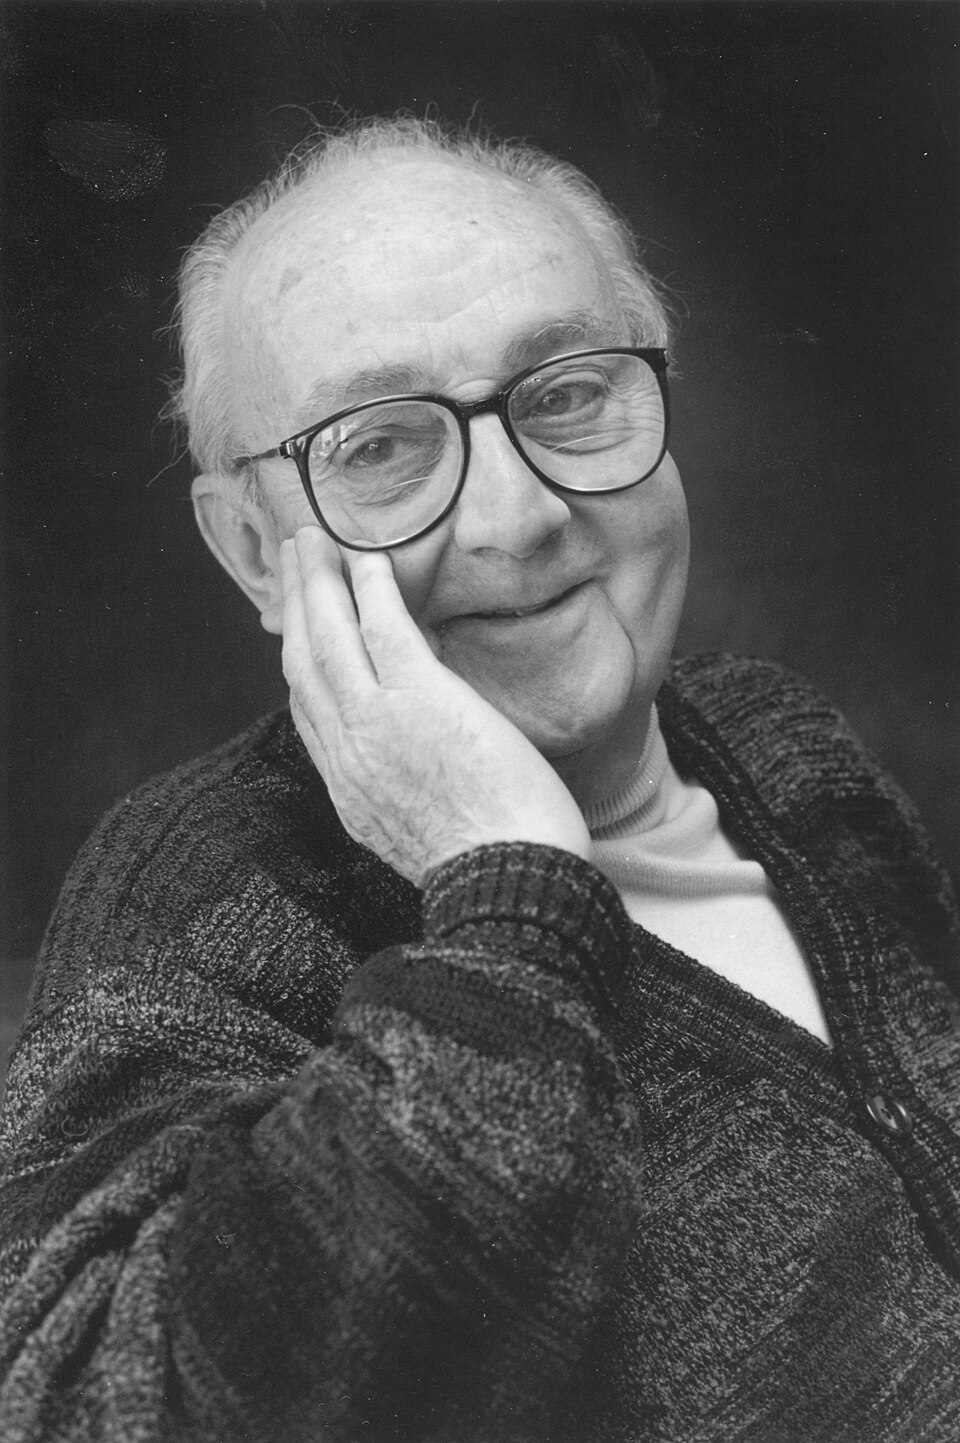
\includegraphics[height=0.46\textheight]{ch6_box.jpg}\\[1mm]
\imgcap{George E. P. Box (1919--2013)}
\imgcredit{https://commons.wikimedia.org/wiki/File:GeorgeEPBox.jpg}{Foto: DavidMCEddy (2011); CC BY-SA 3.0; Wikimedia Commons}
\end{column}
\end{columns}
\end{frame}

\begin{frame}{Șapte distribuții candidate}
\itemsize{\footnotesize}
\begin{center}
\scriptsize
\begin{tabular}{l>{\raggedright\arraybackslash}p{0.8cm}>{\raggedright\arraybackslash}p{3.2cm}>{\raggedright\arraybackslash}p{2.4cm}>{\raggedright\arraybackslash}p{2.6cm}}
\toprule
\textbf{Model} & \textbf{$k$} & \textbf{Cozi} & \textbf{Asimetrie} & \textbf{Referință} \\
\midrule
Normală & 2 & subțiri, $e^{-x^2/2}$ & nu & \sfmchlink{https://danpele.github.io/SFM/RO/Cursuri/capitol2_distributii_clasice_fapte_stilizate.pdf}{Capitolul 2} \\
Student-t & 3 & putere, $x^{-\nu}$ & nu & \sfmchlink{https://danpele.github.io/SFM/RO/Cursuri/capitol2_distributii_clasice_fapte_stilizate.pdf}{Capitolul 2} \\
skewed-t & 4 & putere, $x^{-\nu}$ & da ($\lambda$) & \refHansen{} \\
GED & 3 & $e^{-|x|^\beta}$, groase dacă $\beta < 2$ & nu & \refNelson{} \\
amestec Normal & 5 & subțiri, dar o componentă largă & da & \refKon{} \\
NIG & 4 & semigroase, $|x|^{-3/2}e^{-c|x|}$ & da & \refBN{} \\
stabilă & 4 & putere, $x^{-\alpha}$, $\alpha < 2$ & da ($\beta$) & \sfmchlink{https://danpele.github.io/SFM/RO/Cursuri/capitol3_distributii_alfa_stabile.pdf}{Capitolul 3} \\
\bottomrule
\end{tabular}
\end{center}
\begin{itemize}
    \item $k$: numărul de parametri; GED: generalised error distribution (distribuția erorii generalizate); NIG: normal inverse Gaussian (Normală invers Gaussiană), din familia hiperbolică generalizată \refEK
    \item Amestecul Normal: cu probabilitatea $w$, o zi calmă $N(\mu_1, \sigma_1^2)$, altfel o zi agitată $N(\mu_2, \sigma_2^2)$
\end{itemize}
\end{frame}

\begin{frame}{Candidații comparați}
\itemsize{\footnotesize}
\begin{center}
    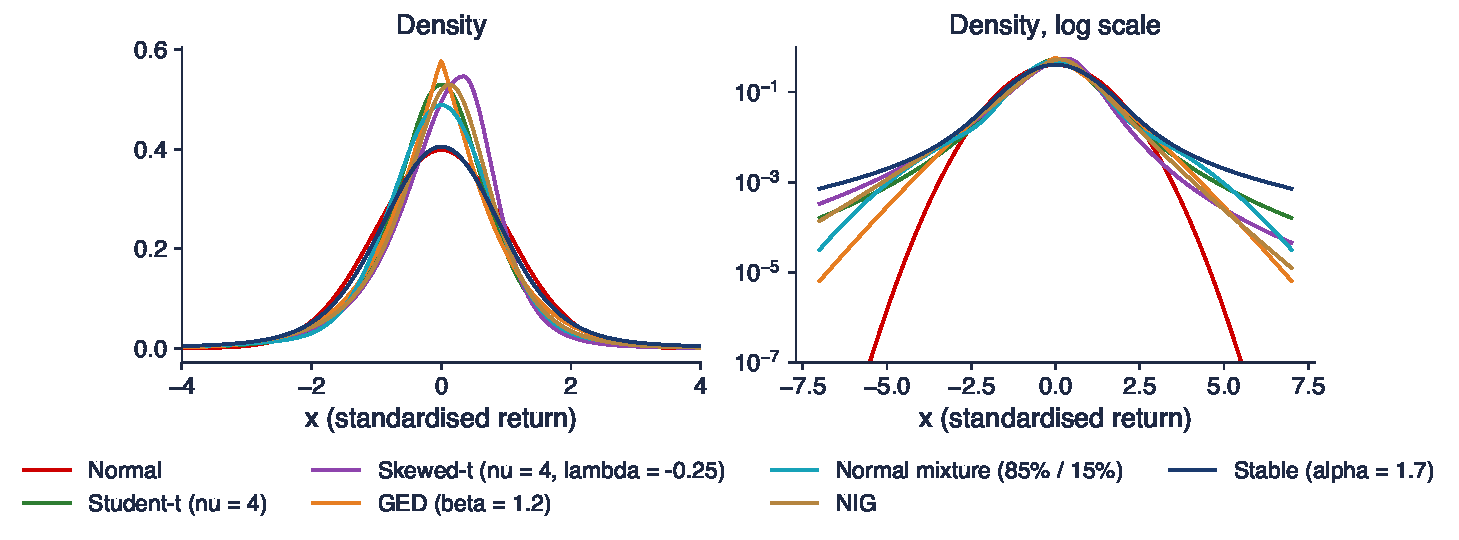
\includegraphics[width=0.97\textwidth,height=0.58\textheight,keepaspectratio]{sfm_ch6_candidates.pdf}
\end{center}
\vspace{-0.25cm}
\begin{itemize}
    \item Toate au media 0 și varianța 1 (distribuția stabilă: același interval intercuartilic ca distribuția Normală); panoul din dreapta folosește scara logaritmică
    \item În centru arată aproape la fel; în cozi diferă cu cîteva ordine de mărime
\end{itemize}
\quantlet{SFM\_ch6\_candidates}{\qlurl{SFM_ch6_candidates}}
\end{frame}

\begin{frame}{Aceeași varianță, cozi foarte diferite}
\itemsize{\small}
\begin{itemize}
    \item $P(X < -4)$, o mișcare de patru abateri standard, pentru fiecare candidat din grafic:
    \begin{itemize}
        \item Normală $3{,}2 \times 10^{-5}$; GED $9{,}5 \times 10^{-4}$; Student-t $2{,}4 \times 10^{-3}$; amestec Normal $2{,}5 \times 10^{-3}$
        \item NIG $3{,}2 \times 10^{-3}$; skewed-t $4{,}5 \times 10^{-3}$; stabilă $8{,}1 \times 10^{-3}$
    \end{itemize}
    \item Distribuția Student-t atribuie acestei pierderi o probabilitate de circa $76$ de ori mai mare decît distribuția Normală
    \item O măsură de risc precum VaR 1\% se află exact în zona în care candidații diferă
    \item \textbf{Întrebare pentru sală}: dacă toate se potrivesc bine în centru, de ce nu îl păstrăm pe cel mai simplu?
    \item \textbf{Răspuns}
    \begin{itemize}
        \item cel mai simplu model (distribuția Normală) greșește exact în zona care determină cerințele de capital și de marjă
    \end{itemize}
\end{itemize}
\end{frame}

\begin{frame}{Statisticile SFESumm: reperele oricărui model}
\itemsize{\footnotesize}
\begin{center}
    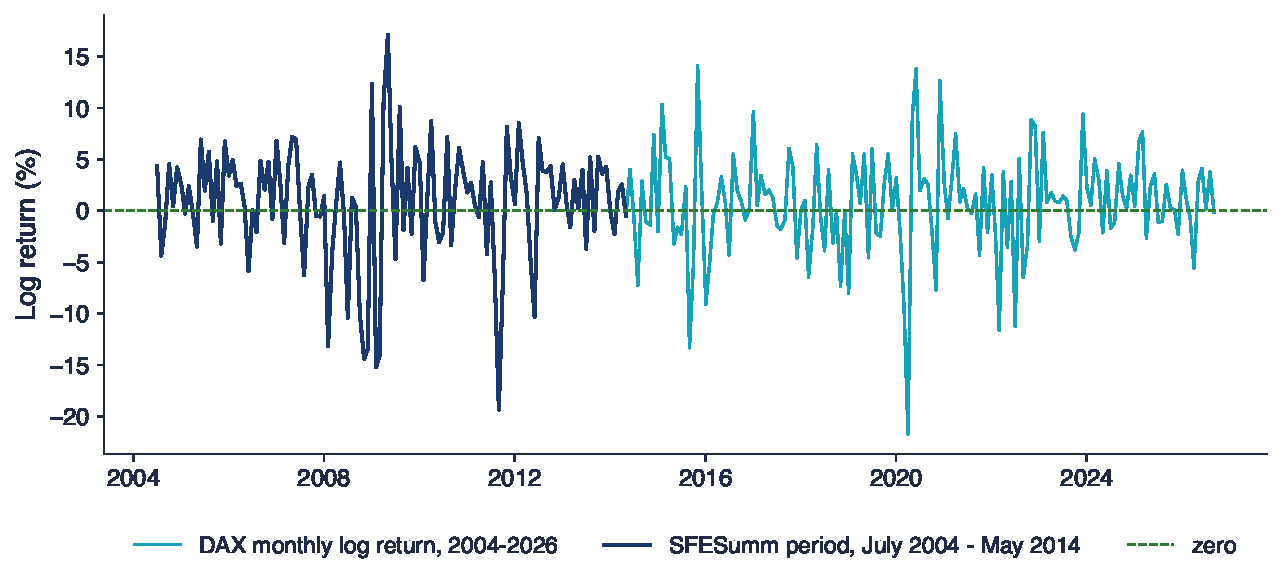
\includegraphics[width=0.97\textwidth,height=0.56\textheight,keepaspectratio]{sfm_ch6_dax_monthly.pdf}
\end{center}
\vspace{-0.25cm}
\begin{itemize}
    \item Quantlet-ul SFESumm: randamentele logaritmice lunare DAX între primele zile de tranzacționare, iulie 2004 -- mai 2014 ($n = 119$), extinse aici pînă la 1 sep. 2026
    \item Chiar și randamentele lunare sînt asimetrice și au cozi groase: cifrele sînt pe slide-ul următor
\end{itemize}
\quantlet{SFM\_ch6\_summary}{\qlurl{SFM_ch6_summary}}
\end{frame}

\begin{frame}{Statistici descriptive: DAX lunar și randamente zilnice}
\itemsize{\footnotesize}
\begin{center}
\footnotesize
\begin{tabular}{lrrrrrrr}
\toprule
& $n$ & min & max & ab.\ std. & vol.\ anuală & asim. & boltire \\
\midrule
DAX 2004--2014 & 119 & $-19{,}35$ & $17{,}12$ & $5{,}80$ & $20{,}08$ & $-0{,}83$ & $4{,}60$ \\
DAX 2004--2026 & 267 & $-21{,}70$ & $17{,}12$ & $5{,}39$ & $18{,}66$ & $-0{,}72$ & $5{,}06$ \\
\bottomrule
\end{tabular}
\end{center}
\begin{itemize}
    \item Lunar, în \%; boltirea (kurtosis) $= E(X - \mu)^4/\sigma^4$, egală cu 3 pentru distribuția Normală; valoarea $p$ Jarque--Bera (\sfmchlink{https://danpele.github.io/SFM/RO/Cursuri/capitol2_distributii_clasice_fapte_stilizate.pdf}{Capitolul 2}) $<0{,}001$
    \item Randamente logaritmice zilnice din 2000 (Bitcoin din 2014, acțiunile BVB din 2010): boltirea
    \begin{itemize}
        \item BET $14{,}1$, S\&P 500 $13{,}7$, DAX $9{,}1$, Bitcoin $15{,}0$, TLV $16{,}5$, SNP $11{,}9$, BRD $10{,}3$
        \item asimetria: S\&P 500 $-0{,}35$, BET $-0{,}65$, Bitcoin $-0{,}70$
    \end{itemize}
\end{itemize}\quantlet{SFM\_ch6\_summary}{\qlurl{SFM_ch6_summary}}
\end{frame}

\begin{frame}{Datele înaintea modelelor: două zile greșite}
\itemsize{\small}
\begin{itemize}
    \item Banca Transilvania (TLV), prețul ajustat de la EODHD: randamente logaritmice de $-15{,}0\%$ pe 30 mai 2016 și $20{,}5\%$ pe 31 mai 2016
    \begin{itemize}
        \item ajustarea pentru acțiunile gratuite este aplicată cu o zi întîrziere (\sfmchlink{https://danpele.github.io/SFM/RO/Cursuri/capitol2_distributii_clasice_fapte_stilizate.pdf}{Capitolul 2}): un crah fals urmat de o creștere falsă
    \end{itemize}
    \item Efectul celor două zile asupra modelului estimat
    \begin{itemize}
        \item boltirea $20{,}5$ cu ele, $16{,}5$ fără; $\hat\nu$ Student-t: $3{,}33$ față de $3{,}44$
        \item clasamentul AIC nu se schimbă aici (cel mai bun: Student-t), dar momentele se schimbă
    \end{itemize}
    \item Regula: înainte de orice selecție de model, comparați cele mai mari randamente cu prețurile de închidere și cu știrile; în restul capitolului, cele două zile sînt eliminate
\end{itemize}
\end{frame}

\begin{frame}{Recapitulare: candidații}
\itemsize{\small}
\begin{itemize}
    \item Șapte candidați cu 2 pînă la 5 parametri; aproape identici în centru, foarte diferiți în cozi
    \item Orice model trebuie să reproducă asimetria și o boltire mult peste 3, chiar și pentru randamentele lunare
    \item Curățați întîi datele: fără cele două prețuri greșite, boltirea TLV scade cu circa $19\%$
\end{itemize}
\end{frame}


%=============================================================================
\section{Recapitulare: metoda verosimilității maxime}
%=============================================================================

\begin{frame}{Verosimilitate și log-verosimilitate}
\itemsize{\small}
\begin{itemize}
    \item Datele $r_1, \dots, r_n$, presupuse i.i.d.\ (independente și identic distribuite), cu densitatea $f(r; \theta)$
    \begin{itemize}
        \item \textbf{verosimilitatea}: $L(\theta) = \prod_{t=1}^n f(r_t; \theta)$, densitatea eșantionului observat, ca funcție de $\theta$
        \item \textbf{log-verosimilitatea}: $\ell(\theta) = \sum_{t=1}^n \ln f(r_t; \theta)$; sumele se manipulează mai ușor decît produsele
    \end{itemize}
    \item \textbf{Estimarea de verosimilitate maximă (ML, maximum likelihood)}: $\hat\theta = \arg\max_\theta \ell(\theta)$
    \begin{itemize}
        \item $\ell(\hat\theta)$, log-verosimilitatea maximizată, stă la baza tuturor comparațiilor din acest capitol
    \end{itemize}
    \item Pentru $n$ mare, $\hat\theta$ are o distribuție aproximativ Normală în jurul valorii adevărate $\theta$, cu covarianța $\approx [-\partial^2\ell/\partial\theta\,\partial\theta^\top]^{-1}$ (inversa informației observate)
\end{itemize}
\end{frame}

\begin{frame}{Exemplu lucrat: modelul Normal, pas cu pas}
\itemsize{\small}
\begin{itemize}
    \item $\ell(\mu, \sigma) = -\dfrac{n}{2}\ln(2\pi\sigma^2) - \dfrac{1}{2\sigma^2}\sum_t (r_t - \mu)^2$
    \begin{itemize}
        \item anulînd derivatele: $\hat\mu = \bar r$, $\hat\sigma^2 = \frac{1}{n}\sum_t (r_t - \bar r)^2$ (numitorul $n$, nu $n - 1$)
        \item înlocuind în $\ell$: $\ell(\hat\theta) = -\dfrac{n}{2}\big[\ln(2\pi\hat\sigma^2) + 1\big]$
    \end{itemize}
    \item S\&P 500, randamente logaritmice zilnice în \%, 2000--2026: $n = 6\,714$, $\hat\mu = 0{,}025$, $\hat\sigma = 1{,}213$
    \begin{itemize}
        \item $\ln(2\pi\hat\sigma^2) = 2{,}2240$, deci $\ell(\hat\theta) = -\frac{6\,714}{2}(2{,}2240 + 1) = -10\,823$
    \end{itemize}
    \item Doar modelul Normal are soluție analitică; celelalte se maximizează numeric
\end{itemize}
\end{frame}

\begin{frame}{Estimarea ML numerică pentru ceilalți candidați (S\&P 500)}
\itemsize{\footnotesize}
\begin{center}
\scriptsize
\begin{tabular}{l>{\raggedright\arraybackslash}p{6.6cm}r}
\toprule
\textbf{Model} & \textbf{Estimări} & $\ell(\hat\theta)$ \\
\midrule
Normală & $\hat\mu = 0{,}025$, $\hat\sigma = 1{,}213$ & $-10\,823$ \\
Student-t & $\hat\nu = 2{,}67$, locație $0{,}068$, scală $0{,}703$ & $-9\,848$ \\
skewed-t & $\hat\nu = 2{,}69$, $\hat\lambda = -0{,}067$, $\hat\mu = 0{,}024$, $\hat\sigma = 1{,}39$ & $-9\,838$ \\
GED & $\hat\beta = 0{,}88$, locație $0{,}068$, scală $0{,}653$ & $-9\,854$ \\
amestec Normal & $\hat w = 79\%$: $N(0{,}089; 0{,}71^2)$; $21\%$: $N(-0{,}223; 2{,}26^2)$ & $-9\,925$ \\
NIG & $\hat a = 0{,}403$, $\hat b = -0{,}048$, locație $0{,}115$, scală $0{,}755$ & $-9\,824$ \\
stabilă & $\hat\alpha = 1{,}540$, $\hat\beta = -0{,}181$, $\hat\gamma = 0{,}582$, $\hat\delta_0 = 0{,}093$ & $-9\,893$ \\
\bottomrule
\end{tabular}
\end{center}
\begin{itemize}
    \item Algoritmul de optimizare: Nelder--Mead aplicat parametrilor transformați (de exemplu $\ln\sigma$, $\ln(\nu - 2)$); amestecul Normal prin algoritmul EM (expectation--maximisation); densitatea stabilă prin FFT (\sfmchlink{https://danpele.github.io/SFM/RO/Cursuri/capitol3_distributii_alfa_stabile.pdf}{Capitolul 3})
    \item Skewed-t: $\mu$ și $\sigma$ sînt media și abaterea standard (parametrizarea lui Hansen)
\end{itemize}\quantlet{SFM\_ch6\_ml\_fits}{\qlurl{SFM_ch6_ml_fits}}
\end{frame}

\begin{frame}{Interpretarea estimărilor}
\itemsize{\small}
\begin{itemize}
    \item Student-t $\hat\nu = 2{,}67$: cozi de tip $x^{-2{,}67}$; varianța există ($\nu > 2$), boltirea nu există ($\nu < 4$)
    \begin{itemize}
        \item boltirea de selecție $13{,}7$ estimează o mărime care, conform modelului estimat, este infinită
    \end{itemize}
    \item Skewed-t $\hat\lambda = -0{,}067 < 0$: o coadă stîngă puțin mai lungă (crahuri)
    \item GED $\hat\beta = 0{,}88$: sub 2 (Normală) și chiar sub 1 (Laplace): un vîrf ascuțit
    \item Amestecul Normal: $79\%$ zile calme cu abaterea standard $0{,}71\%$, $21\%$ zile agitate cu $2{,}26\%$ și medie negativă
    \item Distribuția stabilă, $\hat\alpha = 1{,}540$ (\sfmchlink{https://danpele.github.io/SFM/RO/Cursuri/capitol3_distributii_alfa_stabile.pdf}{Capitolul 3}): cozi mai groase decît orice alt candidat
\end{itemize}
\end{frame}

\begin{frame}{Cît de precis este $\hat\nu$? Log-verosimilitatea profil}
\itemsize{\footnotesize}
\begin{center}
    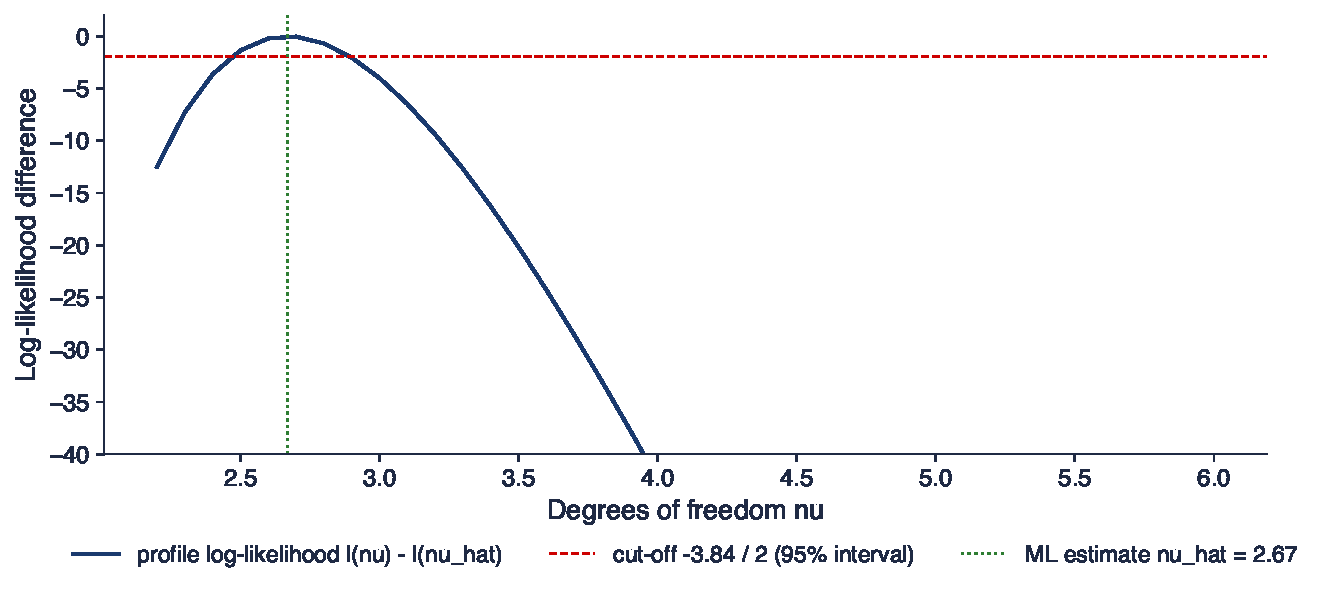
\includegraphics[width=0.97\textwidth,height=0.56\textheight,keepaspectratio]{sfm_ch6_profile_nu.pdf}
\end{center}
\vspace{-0.25cm}
\begin{itemize}
    \item Pentru fiecare $\nu$, maximizăm $\ell$ în raport cu locația și scala; la $\nu = 5$, curba scade cu $-92$
    \item Intervalul de încredere de 95\%: toate valorile $\nu$ pentru care $2[\ell(\hat\nu) - \ell(\nu)] \le 3{,}84$, aici $[2{,}5; 2{,}8]$ în jurul lui $\hat\nu = 2{,}67$: grosimea cozilor este estimată precis
\end{itemize}
\quantlet{SFM\_ch6\_ml\_fits}{\qlurl{SFM_ch6_ml_fits}}
\end{frame}

\begin{frame}{Capcanele ML numerice}
\itemsize{\small}
\begin{itemize}
    \item \textbf{Maxime locale}: optimizatorul se poate opri pe un deal care nu este cel mai înalt
    \begin{itemize}
        \item remediu: mai multe valori inițiale (amestecurile din acest capitol folosesc între 4 și 12 puncte de pornire)
    \end{itemize}
    \item \textbf{Frontiere}: $\nu \to 2$, o pondere a amestecului $\to 0$, $|\lambda| \to 1$
    \begin{itemize}
        \item erorile standard și testele obișnuite nu sînt valide la frontieră (secțiunea următoare)
    \end{itemize}
    \item \textbf{Parametrizarea}: aceeași distribuție, parametrizări diferite
    \begin{itemize}
        \item scala Student-t din scipy nu este abaterea standard: $\mathrm{sd} = \mathrm{scale}\sqrt{\nu/(\nu - 2)}$
    \end{itemize}
    \item \textbf{Verificare}: comparați $\ell(\hat\theta)$ pentru modelele imbricate; un model mai general nu poate avea un maxim mai mic
\end{itemize}
\end{frame}

\begin{frame}{Recapitulare: verosimilitatea maximă}
\itemsize{\small}
\begin{itemize}
    \item $\ell(\theta) = \sum_t \ln f(r_t; \theta)$; estimarea ML o maximizează
    \item Normală: soluție analitică, $\ell(\hat\theta) = -\frac{n}{2}[\ln(2\pi\hat\sigma^2) + 1]$; celelalte: numeric
    \item Precizia rezultă din curbura lui $\ell$ sau din log-verosimilitatea profil
    \item Atenție la maxime locale, frontiere și parametrizări
\end{itemize}
\end{frame}


%=============================================================================
\section{Modele imbricate: testul raportului de verosimilitate}
%=============================================================================

\begin{frame}{Modele imbricate}
\itemsize{\small}
\begin{itemize}
    \item Modelul 0 este \textbf{imbricat} în modelul 1 dacă modelul 0 este modelul 1 cu unii parametri fixați
    \begin{itemize}
        \item Normală în GED: $\beta = 2$
        \item Student-t în skewed-t: $\lambda = 0$
        \item Normală în Student-t: $\nu = \infty$, adică $1/\nu = 0$, la \textbf{marginea} spațiului parametrilor
    \end{itemize}
    \item Neimbricate: Student-t și GED, Student-t și stabilă, skewed-t și NIG
    \begin{itemize}
        \item niciunul nu este caz particular al celuilalt: sînt necesare alte instrumente (testul Vuong, AIC)
    \end{itemize}
    \item Modele imbricate: întotdeauna $\ell_1(\hat\theta_1) \ge \ell_0(\hat\theta_0)$; întrebarea este dacă cîștigul depășește ce s-ar obține din întîmplare
\end{itemize}
\end{frame}

\begin{frame}{Testul raportului de verosimilitate}
\itemsize{\small}
\begin{itemize}
    \item $H_0$: modelul 0 (restrîns) este adevărat; $H_1$: modelul 1 (mai general)
    \begin{itemize}
        \item $LR = 2\,[\ell_1(\hat\theta_1) - \ell_0(\hat\theta_0)] \ge 0$
        \item \textbf{Teorema lui Wilks} (\refWilks): sub $H_0$, $LR \approx \chi^2(d)$, cu $d = k_1 - k_0$ restricții, dacă valorile fixate se află în interiorul spațiului parametrilor
    \end{itemize}
    \item Decizia la 5\%: respingem $H_0$ dacă $LR > \chi^2_{0{,}95}(d)$
    \begin{itemize}
        \item $\chi^2_{0{,}95}(1) = 3{,}84$; $\chi^2_{0{,}95}(2) = 5{,}99$
    \end{itemize}
    \item Intuiția: de două ori logaritmul raportului dintre verosimilitățile datelor sub cele două modele
\end{itemize}
\end{frame}

\begin{frame}{Exemplu lucrat: este necesar parametrul de asimetrie?}
\itemsize{\small}
\begin{itemize}
    \item S\&P 500: $\ell$(Student-t) $= -9\,848$, $\ell$(skewed-t) $= -9\,838$
    \begin{itemize}
        \item $LR = 2(-9\,838 - (-9\,848)) = 19{,}63 > 3{,}84$; $p <0{,}001$: respingem $\lambda = 0$
    \end{itemize}
    \item Același test pentru alte serii
    \begin{itemize}
        \item DAX: $LR = 20{,}92$, $p <0{,}001$: asimetria este necesară
        \item BET: $LR = 0{,}35$, $p = 0{,}555$; Bitcoin: $LR = 0{,}42$, $p = 0{,}515$: nicio dovadă de asimetrie
    \end{itemize}
    \item Normală în GED ($\beta = 2$): $LR$ între 1\,431 (Bitcoin) și 2\,298 (BET); modelul Normal este respins peste tot
    \item Interpretare: cei doi indici dezvoltați au o coadă stîngă mai lungă; BET și Bitcoin nu
\end{itemize}\quantlet{SFM\_ch6\_lr\_aic}{\qlurl{SFM_ch6_lr_aic}}
\end{frame}

\begin{frame}{Un caz de frontieră: Normală în Student-t}
\itemsize{\small}
\begin{itemize}
    \item $H_0$: $1/\nu = 0$ este pe marginea spațiului $1/\nu \ge 0$: teorema lui Wilks nu se aplică
    \begin{itemize}
        \item \refSL: distribuția statisticii sub $H_0$ este un amestec 50:50 de $\chi^2(0)$ (o masă de probabilitate concentrată în 0) și $\chi^2(1)$
        \item valoarea critică la 5\%: $\chi^2_{0{,}90}(1) = 2{,}71$ în loc de $3{,}84$; valoarea $p$ naivă este dublul celei corecte
    \end{itemize}
    \item Date reale: $LR$ = 1\,949 (S\&P 500), 1\,337 (Bitcoin): modelul Normal este respins cu oricare valoare critică
    \item Aceeași problemă apare pentru o pondere a amestecului $w = 0$ și pentru parametri de varianță egali cu 0
    \item \textbf{Ce credeți?} Contează frontiera cînd $LR$ este de ordinul miilor?
    \item \textbf{Răspuns}
    \begin{itemize}
        \item nu pentru decizia de aici; contează însă în eșantioane mici și pentru valori $LR$ la limită, unde înjumătățește valoarea $p$
    \end{itemize}
\end{itemize}
\end{frame}

\begin{frame}{Modele neimbricate: testul Vuong}
\itemsize{\footnotesize}
\begin{center}
\footnotesize
\begin{tabular}{lrrr}
\toprule
& Student-t față de GED & Student-t față de stabilă & skewed-t față de NIG \\
\midrule
BET & $3{,}70$ ($<0{,}001$) & $9{,}33$ ($<0{,}001$) & $-1{,}34$ ($0{,}179$) \\
S\&P 500 & $0{,}40$ ($0{,}686$) & $6{,}52$ ($<0{,}001$) & $-2{,}20$ ($0{,}028$) \\
DAX & $-0{,}23$ ($0{,}817$) & $7{,}66$ ($<0{,}001$) & $-2{,}97$ ($0{,}003$) \\
Bitcoin & $-3{,}80$ ($<0{,}001$) & $16{,}47$ ($<0{,}001$) & $-6{,}76$ ($<0{,}001$) \\
\bottomrule
\end{tabular}
\end{center}
\begin{itemize}
    \item \refVuong: $m_t = \ln f_1(r_t) - \ln f_2(r_t)$, $V = \sqrt{n}\,\bar m / s_m \approx N(0, 1)$ dacă ambele modele sînt la fel de aproape de adevăr
    \item $V > 1{,}96$: primul model este mai aproape; $V < -1{,}96$: al doilea; valoarea $p$ este în paranteză
    \item Student-t este preferat distribuției stabile pe toate piețele; NIG este preferat distribuției skewed-t pentru S\&P 500 și DAX; comparația Student-t--GED diferă de la o piață la alta
\end{itemize}\quantlet{SFM\_ch6\_lr\_aic}{\qlurl{SFM_ch6_lr_aic}}
\end{frame}

\begin{frame}{Recapitulare: testele raportului de verosimilitate și Vuong}
\itemsize{\small}
\begin{itemize}
    \item Modele imbricate: $LR = 2(\ell_1 - \ell_0) \approx \chi^2(k_1 - k_0)$ (Wilks)
    \item La frontieră (Normală în Student-t): amestec 50:50, valoarea critică $2{,}71$
    \item Modele neimbricate: testul Vuong pe diferențele punctuale de log-verosimilitate
    \item Asimetria contează pentru S\&P 500 și DAX, nu pentru BET și Bitcoin
\end{itemize}
\end{frame}


%=============================================================================
\section{Criterii informaționale: AIC și BIC}
%=============================================================================

\begin{frame}{Ideea lui Akaike}
\itemsize{\small}
\begin{columns}[T]
\begin{column}{0.64\textwidth}
\begin{itemize}
    \item Hirotugu Akaike și-a pus întrebarea: ce model va prezice cel mai bine date \textbf{noi}?
    \begin{itemize}
        \item distanța de la distribuția adevărată $g$ la un model $f$: divergența Kullback--Leibler \refKL
        \item $KL(g, f) = E_g[\ln g(R) - \ln f(R)] \ge 0$, zero doar dacă $f = g$
    \end{itemize}
    \item $\ell(\hat\theta)$ este prea optimistă: aceleași date servesc și la estimarea lui $\hat\theta$, și la evaluarea lui
    \begin{itemize}
        \item supraestimarea este, în medie, de circa $k$, numărul de parametri \refAkaike
    \end{itemize}
    \item Rezultatul: $\mathrm{AIC} = -2\ell(\hat\theta) + 2k$, o estimare a calității ajustării așteptate în afara eșantionului (valoarea mai mică este preferată)
\end{itemize}
\end{column}
\begin{column}{0.32\textwidth}
\centering
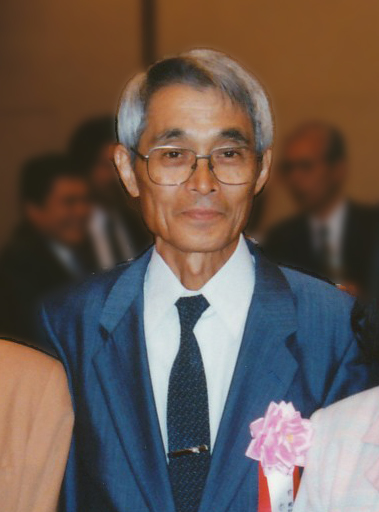
\includegraphics[height=0.44\textheight]{ch6_akaike.jpg}\\[1mm]
\imgcap{Hirotugu Akaike (1927--2009)}
\imgcredit{https://commons.wikimedia.org/wiki/File:Akaike.jpg}{Foto: The Institute of Statistical Mathematics; CC BY-SA 4.0; Wikimedia Commons}
\end{column}
\end{columns}
\end{frame}

\begin{frame}{AIC și BIC}
\itemsize{\small}
\begin{itemize}
    \item \textbf{AIC} (Akaike information criterion, criteriul informațional Akaike): $\mathrm{AIC} = -2\ell(\hat\theta) + 2k$
    \begin{itemize}
        \item scopul: cel mai bun model predictiv; asimptotic echivalent cu validarea încrucișată leave-one-out \refStone
        \item eșantioane mici: AICc $= \mathrm{AIC} + 2k(k+1)/(n - k - 1)$ \refHT
    \end{itemize}
    \item \textbf{BIC} (Bayesian information criterion, criteriul informațional bayesian) \refSchwarz: $\mathrm{BIC} = -2\ell(\hat\theta) + k\ln n$
    \begin{itemize}
        \item scopul: modelul adevărat, dacă este printre candidați (consistență)
        \item penalizarea pe parametru $\ln n$: $8{,}81$ pentru $n = 6\,714$, de peste patru ori mai mare decît penalizarea AIC, egală cu 2
    \end{itemize}
    \item Pentru ambele criterii, valoarea mai mică este preferată; doar diferențele dintre modele estimate pe \textbf{aceleași date} sînt interpretabile
\end{itemize}
\end{frame}

\begin{frame}{$\Delta$AIC și ponderile Akaike}
\itemsize{\small}
\begin{itemize}
    \item $\Delta_i = \mathrm{AIC}_i - \min_j \mathrm{AIC}_j$; regulile practice din \refBA:
    \begin{itemize}
        \item $\Delta \le 2$: sprijin substanțial; $4 \le \Delta \le 7$: considerabil mai puțin; $\Delta > 10$: practic niciunul
    \end{itemize}
    \item \textbf{Ponderea Akaike}: $w_i = \dfrac{e^{-\Delta_i/2}}{\sum_j e^{-\Delta_j/2}}$
    \begin{itemize}
        \item ponderea dovezilor în favoarea modelului $i$ dintre candidați; suma ponderilor este 1
        \item două modele cu $\Delta = 0$ și $\Delta = 2$: $w = 1/(1 + e^{-1}) \approx 0{,}73$ și $0{,}27$
    \end{itemize}
    \item \textbf{Ce credeți?} Este $\Delta = 2$ o diferență „semnificativă”?
    \item \textbf{Răspuns}
    \begin{itemize}
        \item nu: AIC nu este un test; o diferență de 2 înseamnă că ambele modele rămîn plauzibile (circa 73\% față de 27\%)
    \end{itemize}
\end{itemize}
\end{frame}

\begin{frame}{Exemplu lucrat: șapte modele pentru S\&P 500}
\itemsize{\footnotesize}
\begin{center}
\scriptsize
\begin{tabular}{lrrrrrrr}
\toprule
& $k$ & $\ell(\hat\theta)$ & AIC & BIC & $\Delta$AIC & $\Delta$BIC & $w$ \\
\midrule
Normală & 2 & $-10\,823$ & $21\,650$ & $21\,663$ & $1993{,}2$ & $1979{,}6$ & $0{,}000$ \\
Student-t & 3 & $-9\,848$ & $19\,702$ & $19\,723$ & $45{,}7$ & $38{,}9$ & $0{,}000$ \\
skewed-t & 4 & $-9\,838$ & $19\,685$ & $19\,712$ & $28{,}1$ & $28{,}1$ & $0{,}000$ \\
GED & 3 & $-9\,854$ & $19\,714$ & $19\,735$ & $57{,}9$ & $51{,}1$ & $0{,}000$ \\
amestec Normal & 5 & $-9\,925$ & $19\,859$ & $19\,893$ & $202{,}5$ & $209{,}3$ & $0{,}000$ \\
NIG & 4 & $-9\,824$ & $19\,657$ & $19\,684$ & $0{,}0$ & $0{,}0$ & $1{,}000$ \\
stabilă & 4 & $-9\,893$ & $19\,794$ & $19\,821$ & $137{,}3$ & $137{,}3$ & $0{,}000$ \\
\bottomrule
\end{tabular}
\end{center}
\begin{itemize}
    \item Exemplu: NIG, $\mathrm{AIC} = -2(-9\,824) + 2 \cdot 4 = 19\,657$
    \item NIG cîștigă pe ambele criterii; următorul model, skewed-t, are $\Delta = 28{,}1$, deci $e^{-\Delta/2} \approx 8{,}1 \times 10^{-7}$: ponderea $w \approx 1$ pentru NIG
    \item modelul Normal: $\Delta$AIC de 1\,993; distribuția stabilă: 137
\end{itemize}\quantlet{SFM\_ch6\_lr\_aic}{\qlurl{SFM_ch6_lr_aic}}
\end{frame}

\begin{frame}{$\Delta$AIC pentru șapte serii}
\itemsize{\footnotesize}
\begin{center}
    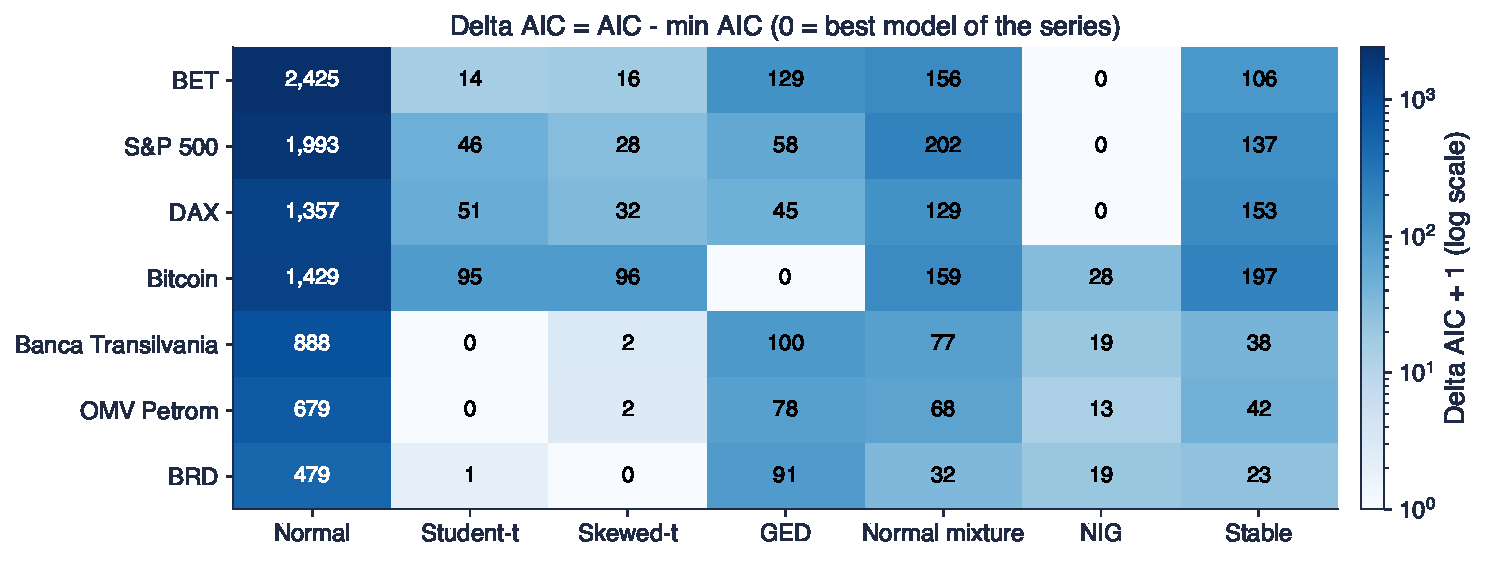
\includegraphics[width=0.97\textwidth,height=0.62\textheight,keepaspectratio]{sfm_ch6_delta_aic.pdf}
\end{center}
\vspace{-0.25cm}
\begin{itemize}
    \item Fiecare rînd: o serie; 0 marchează cel mai bun model; celule mai închise: modele mai slabe (scară logaritmică a culorii)
\end{itemize}
\quantlet{SFM\_ch6\_lr\_aic}{\qlurl{SFM_ch6_lr_aic}}
\end{frame}

\begin{frame}{Interpretarea hărții $\Delta$AIC}
\itemsize{\small}
\begin{itemize}
    \item Niciun cîștigător unic: cel mai bun model depinde de piață
    \begin{itemize}
        \item indicii (BET, S\&P 500, DAX): NIG; Bitcoin: GED; acțiunile BVB: Student-t (TLV, SNP) și skewed-t (BRD)
    \end{itemize}
    \item Concluzii robuste
    \begin{itemize}
        \item modelul Normal este ultimul peste tot, cu $\Delta$AIC între 479 (BRD) și 2\,425 (BET)
        \item distribuția stabilă ($\Delta$ de la 23 la 197) și amestecul Normal nu sînt niciodată competitive
    \end{itemize}
    \item \textbf{Întrebare pentru sală}: pentru BRD, AIC preferă skewed-t ($\Delta$ al Student-t: $1{,}0$); ce model preferă BIC?
    \item \textbf{Răspuns}
    \begin{itemize}
        \item Student-t: un parametru în minus reduce BIC cu $\ln n \approx 8{,}2$, mai mult decît cîștigul de ajustare; cu $\Delta \approx 1$, cele două sînt practic la egalitate
    \end{itemize}
\end{itemize}
\end{frame}

\begin{frame}{Recapitulare: criteriile informaționale}
\itemsize{\small}
\begin{itemize}
    \item AIC $= -2\ell + 2k$ (predicție); BIC $= -2\ell + k\ln n$ (modelul adevărat, penalizare mai mare)
    \item Citiți $\Delta$AIC și ponderile Akaike, nu nivelul AIC; $\Delta \le 2$ înseamnă practic egalitate
    \item Indici: NIG; Bitcoin: GED; acțiuni BVB: Student-t; Normală și stabilă: niciodată
    \item AIC ordonează candidații; nu spune dacă cel mai bun este suficient de bun
\end{itemize}
\end{frame}


%=============================================================================
\section{Teste de concordanță}
%=============================================================================

\begin{frame}{De la Pearson la funcția de repartiție empirică}
\itemsize{\small}
\begin{columns}[T]
\begin{column}{0.64\textwidth}
\begin{itemize}
    \item \refPearson: primul test de concordanță, testul $\chi^2$
    \begin{itemize}
        \item grupăm datele în clase și comparăm frecvențele observate cu cele așteptate
        \item rezultatul depinde de clase, iar cozile conțin puține observații
    \end{itemize}
    \item \textbf{Funcția de repartiție empirică} (EDF, empirical distribution function): $F_n(x) = \frac{1}{n}\#\{t: r_t \le x\}$
    \begin{itemize}
        \item fără clase: comparăm $F_n$ cu funcția de repartiție a modelului $F$
    \end{itemize}
    \item Trei teste EDF: Kolmogorov--Smirnov, Cramér--von Mises, Anderson--Darling \refStephens
\end{itemize}
\end{column}
\begin{column}{0.32\textwidth}
\centering
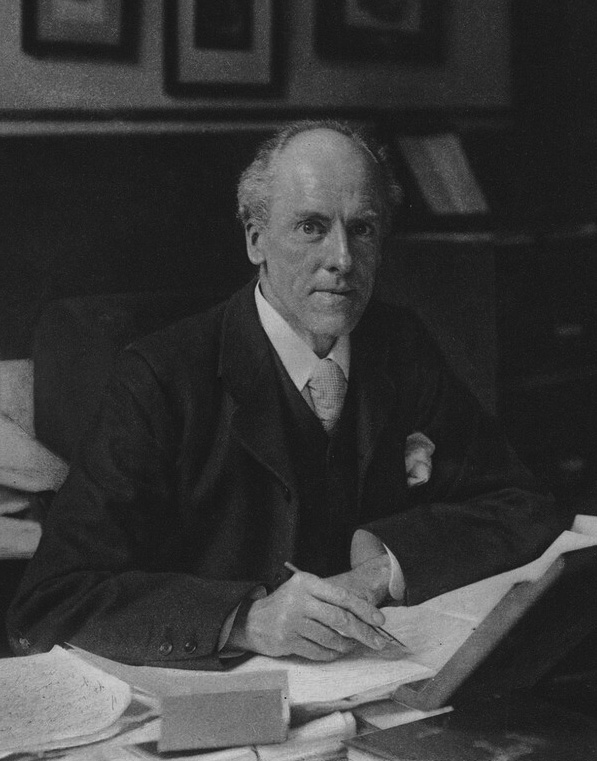
\includegraphics[height=0.44\textheight]{ch6_pearson.jpg}\\[1mm]
\imgcap{Karl Pearson (1857--1936)}
\imgcredit{https://commons.wikimedia.org/wiki/File:Karl_Pearson.jpg}{Fotogravură (1910); domeniu public; Wikimedia Commons}
\end{column}
\end{columns}
\end{frame}

\begin{frame}{Testul Kolmogorov--Smirnov}
\itemsize{\small}
\begin{columns}[T]
\begin{column}{0.6\textwidth}
\begin{itemize}
    \item $D_n = \sup_x |F_n(x) - F(x)|$, cea mai mare distanță pe verticală
    \begin{itemize}
        \item cu datele ordonate $u_{(i)} = F(r_{(i)})$: $D_n = \max_i \max\{i/n - u_{(i)},\ u_{(i)} - (i-1)/n\}$
    \end{itemize}
    \item $F$ complet cunoscută: distribuția lui $D_n$ nu depinde de $F$ (Kolmogorov, 1933)
    \begin{itemize}
        \item $n$ mare: respingem la 5\% dacă $D_n > 1{,}358/\sqrt{n}$; tabele pentru $n$ mic: \refSmirnov
        \item $n = 6\,714$: valoarea critică $0{,}017$
    \end{itemize}
    \item Andrei Kolmogorov este și autorul axiomaticii probabilităților (\sfmchlink{https://danpele.github.io/SFM/RO/Cursuri/capitol4_probabilitate.pdf}{Capitolul 4})
\end{itemize}
\end{column}
\begin{column}{0.36\textwidth}
\centering
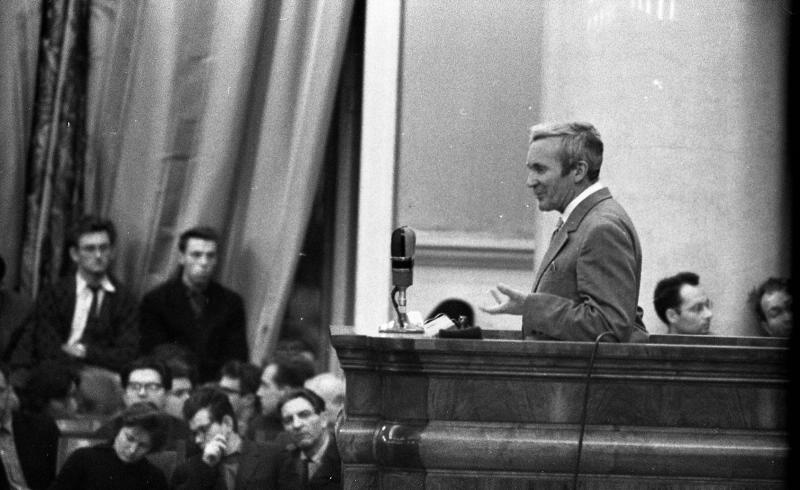
\includegraphics[height=0.38\textheight]{ch4_kolmogorov_1963.jpg}\\[1mm]
\imgcap{Andrei Kolmogorov (1903--1987) la curs, 1963}
\imgcredit{https://commons.wikimedia.org/wiki/File:Математик_Андрей_Колмогоров_в_аудитории.jpg}{Foto: Vsevolod Tarasevich (1963--1964); CC BY 4.0; Wikimedia Commons}
\end{column}
\end{columns}
\end{frame}

\begin{frame}{Exemplu lucrat: KS pe cinci randamente}
\itemsize{\small}
\begin{itemize}
    \item Randamente (\%): $-2{,}1;\ -0{,}4;\ 0{,}3;\ 0{,}9;\ 1{,}6$; $H_0$: $N(0, 1)$, complet specificată
    \begin{itemize}
        \item $u_{(i)} = \Phi(r_{(i)})$: $0{,}018$; $0{,}345$; $0{,}618$; $0{,}816$; $0{,}945$ ($\Phi$: funcția de repartiție Normală standard)
        \item $i/n$: $0{,}2;\ 0{,}4;\ 0{,}6;\ 0{,}8;\ 1{,}0$; cea mai mare distanță este $u_{(3)} - 2/5 = 0{,}218$
    \end{itemize}
    \item $D_5 = 0{,}218 < 0{,}563$, valoarea critică exactă la 5\% pentru $n = 5$: nu respingem
    \item Cu cinci observații, aproape orice distribuție trece testul: în eșantioane mici, puterea testului este redusă
\end{itemize}\quantlet{SFM\_ch6\_gof\_tests}{\qlurl{SFM_ch6_gof_tests}}
\end{frame}

\begin{frame}{Parametri estimați: problema Lilliefors}
\itemsize{\small}
\begin{itemize}
    \item În practică, $F$ are parametri estimați: $F(x; \hat\theta)$ este estimată pe aceleași date
    \begin{itemize}
        \item estimarea apropie $F$ de $F_n$: $D_n$ este mai mic decît pentru o $F$ cunoscută
        \item valorile critice obișnuite sînt prea mari: testul aproape că nu mai respinge
    \end{itemize}
    \item \refLilliefors: valori critice obținute prin simulare pentru distribuția Normală cu $\hat\mu$, $\hat\sigma$ (nivelul 5\%)
    \begin{itemize}
        \item $n = 5$: $0{,}351$ în loc de $0{,}563$; $n = 1000$: $0{,}029$ în loc de $0{,}043$
    \end{itemize}
    \item Orice model: \textbf{bootstrap parametric} \refSGQ
    \begin{itemize}
        \item simulăm $n$ extrageri din $F(\cdot; \hat\theta)$, reestimăm parametrii, recalculăm statistica; repetăm de $B$ ori
        \item valoarea $p$ $= (1 + \#\{\text{statistici bootstrap} \ge \text{cea observată}\})/(B + 1)$
    \end{itemize}
\end{itemize}
\end{frame}

\begin{frame}{Cramér--von Mises și Anderson--Darling}
\itemsize{\small}
\begin{columns}[T]
\begin{column}{0.66\textwidth}
\begin{itemize}
    \item Ambele integrează pătratul distanței $[F_n(x) - F(x)]^2$ pe toate valorile $x$ în loc să ia maximul
    \begin{itemize}
        \item \textbf{Cramér--von Mises}: $W^2 = n\int [F_n - F]^2\, dF = \frac{1}{12n} + \sum_i \big(u_{(i)} - \frac{2i - 1}{2n}\big)^2$ \refCramer
        \item \textbf{Anderson--Darling}: $A^2 = n\int \dfrac{[F_n - F]^2}{F(1 - F)}\, dF$ \refAD
    \end{itemize}
    \item Formula de calcul \refADb: $A^2 = -n - \frac{1}{n}\sum_i (2i - 1)\big[\ln u_{(i)} + \ln(1 - u_{(n + 1 - i)})\big]$
    \begin{itemize}
        \item ponderea $1/[F(1 - F)]$ este foarte mare acolo unde $F$ este aproape de 0 sau 1, adică în cozi
    \end{itemize}
\end{itemize}
\end{column}
\begin{column}{0.30\textwidth}
\centering
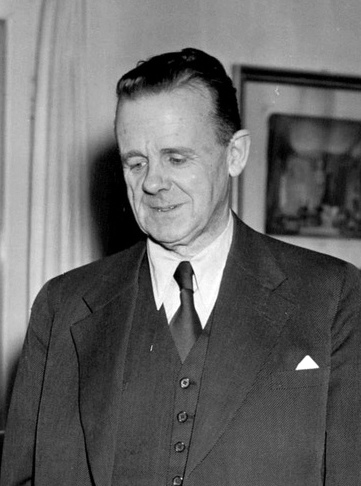
\includegraphics[height=0.42\textheight]{ch6_cramer.jpg}\\[1mm]
\imgcap{Harald Cramér (1893--1985)}
\imgcredit{https://commons.wikimedia.org/wiki/File:Harald_Cramér.jpg}{Foto: fotograf necunoscut (1951); domeniu public; Wikimedia Commons}
\end{column}
\end{columns}
\end{frame}

\begin{frame}{De ce este KS slab în cozi}
\itemsize{\footnotesize}
\begin{center}
    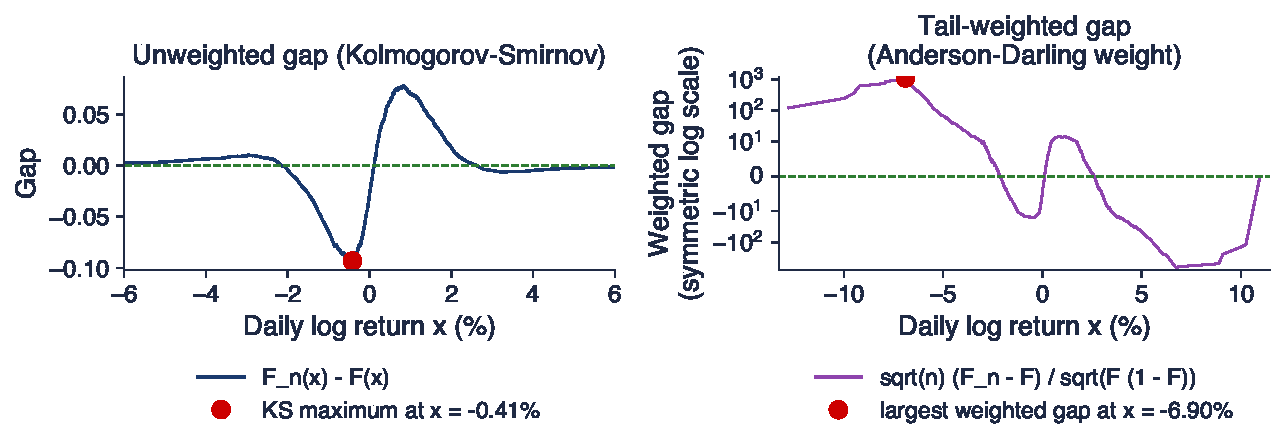
\includegraphics[width=0.97\textwidth,height=0.54\textheight,keepaspectratio]{sfm_ch6_ks_tail.pdf}
\end{center}
\vspace{-0.25cm}
\begin{itemize}
    \item S\&P 500 comparat cu distribuția Normală estimată. Stînga: distanța KS are maximul la $x = -0{,}41\%$, aproape de centru ($F = 36\%$), cu $D_n = 0{,}093$
    \item În cozi, $F_n$ și $F$ sînt amîndouă aproape de 0 sau 1, deci distanța brută este mică chiar dacă modelul greșește mult; cu ponderea Anderson--Darling (dreapta), distanța maximă apare la $x = -6{,}9\%$
\end{itemize}
\quantlet{SFM\_ch6\_gof\_tests}{\qlurl{SFM_ch6_gof_tests}}
\end{frame}

\begin{frame}{Puterea celor trei teste}
\itemsize{\footnotesize}
\begin{center}
    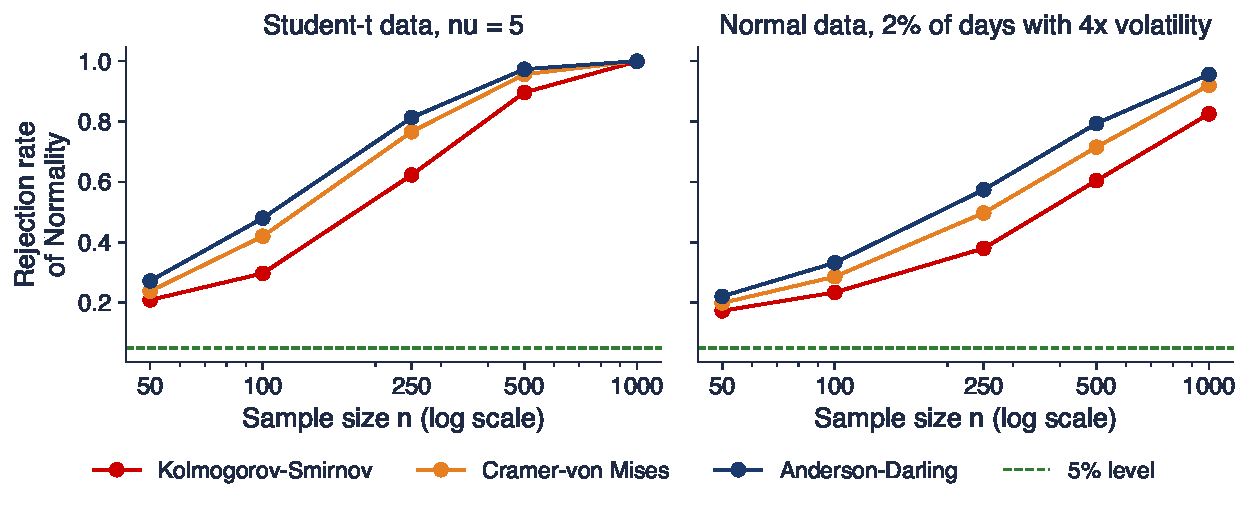
\includegraphics[width=0.97\textwidth,height=0.54\textheight,keepaspectratio]{sfm_ch6_gof_power.pdf}
\end{center}
\vspace{-0.25cm}
\begin{itemize}
    \item Proporția din 1000 de eșantioane simulate în care normalitatea (parametri estimați) este respinsă la 5\%; puterea = probabilitatea de a respinge un $H_0$ fals
    \item Date Student-t, $n = 250$: KS $62\%$, Cramér--von Mises $77\%$, Anderson--Darling $81\%$; abateri doar în cozi ($n = 250$): $38\%$, $50\%$, $57\%$
\end{itemize}
\quantlet{SFM\_ch6\_gof\_tests}{\qlurl{SFM_ch6_gof_tests}}
\end{frame}

\begin{frame}{Teste EDF pe S\&P 500}
\itemsize{\footnotesize}
\begin{columns}[T]
\begin{column}{0.44\textwidth}
\begin{center}
\scriptsize
\begin{tabular}{lrrr}
\toprule
& KS & CvM & AD \\
\midrule
Normală & $0{,}093$ & $22{,}84$ & $127{,}35$ \\
Student-t & $0{,}018$ & $0{,}57$ & $4{,}69$ \\
skewed-t & $0{,}017$ & $0{,}41$ & $2{,}25$ \\
GED & $0{,}019$ & $0{,}38$ & $3{,}94$ \\
amestec Normal & $0{,}025$ & $1{,}09$ & $5{,}80$ \\
NIG & $0{,}010$ & $0{,}13$ & $0{,}88$ \\
stabilă & $0{,}022$ & $0{,}81$ & $4{,}61$ \\
\bottomrule
\end{tabular}
\end{center}

\end{column}
\begin{column}{0.52\textwidth}
\begin{itemize}
    \item Bootstrap parametric, $B = 199$, valori critice (cuantila de 95\%)
    \begin{itemize}
        \item Student-t: KS $0{,}009$, AD $0{,}71$
        \item skewed-t: KS $0{,}008$, AD $0{,}35$
    \end{itemize}
    \item Normală, Student-t, skewed-t: $p$ bootstrap $= 0{,}005$, cel mai mic posibil: toate respinse
    \item Student-t, valoarea $p$ KS naivă (ca și cum $\theta$ ar fi cunoscut): $0{,}021$
\end{itemize}
\end{column}
\end{columns}\begin{itemize}
    \item KS: Kolmogorov--Smirnov; CvM: Cramér--von Mises; AD: Anderson--Darling; valorile mai mici indică o ajustare mai bună
\end{itemize}\quantlet{SFM\_ch6\_gof\_tests}{\qlurl{SFM_ch6_gof_tests}}
\end{frame}

\begin{frame}{Semnificație statistică și semnificație practică}
\itemsize{\small}
\begin{itemize}
    \item Cu $n = 6\,714$, toate modelele sînt respinse: testele detectează abateri minuscule
    \begin{itemize}
        \item în plus, randamentele reale nu sînt i.i.d.\ (volatility clustering), deci nicio distribuție i.i.d.\ nu poate trece testul
    \end{itemize}
    \item Folosiți statisticile pentru a \textbf{ordona} modelele
    \begin{itemize}
        \item AD: Normală $127{,}35$, Student-t $4{,}69$, skewed-t $2{,}25$, NIG $0{,}88$
        \item ca la AIC: NIG pe primul loc, modelul Normal mult în urmă
    \end{itemize}
    \item \textbf{Întrebare pentru sală}: un test KS pe 50 de randamente zilnice nu respinge distribuția Normală; este atunci distribuția Normală potrivită pentru VaR 1\%?
    \item \textbf{Răspuns}
    \begin{itemize}
        \item nu: cu $n = 50$, testul respinge rar chiar și date Student-t (în $30\%$ din cazuri la $n = 100$), iar KS aproape ignoră coada
    \end{itemize}
\end{itemize}
\end{frame}

\begin{frame}{Recapitulare: testele de concordanță}
\itemsize{\small}
\begin{itemize}
    \item KS: cea mai mare distanță; CvM: pătratul distanței, integrat; AD: aceeași mărime, cu pondere mai mare în cozi
    \item Parametri estimați: tabelele Lilliefors sau un bootstrap parametric; niciodată tabelul KS clasic
    \item Puterea: AD > CvM > KS pentru alternative cu cozi groase
    \item Pe eșantioane mari, testele resping orice model: ordonați modelele după statistică și examinați graficele
\end{itemize}
\end{frame}


%=============================================================================
\section{Grafice PP și QQ}
%=============================================================================

\begin{frame}{Două moduri de a evalua vizual ajustarea}
\itemsize{\small}
\begin{itemize}
    \item \textbf{Grafic PP} (probabilitate--probabilitate): punctele $\big(p_i, F(r_{(i)})\big)$ cu $p_i = (i - 0{,}5)/n$
    \begin{itemize}
        \item ambele axe în $[0, 1]$: se văd diferențele din centru; cozile sînt înghesuite în colțuri
        \item echivalentul grafic al testului KS: cea mai mare distanță pe verticală față de diagonală este apropiată de $D_n$
    \end{itemize}
    \item \textbf{Grafic QQ} (cuantilă--cuantilă): punctele $\big(F^{-1}(p_i), r_{(i)}\big)$
    \begin{itemize}
        \item în unități de randament: cozile sînt dilatate, iar fiecare zi extremă este vizibilă
        \item capetele se îndepărtează de dreaptă: cozile modelului sînt prea scurte; capetele aplatizate: cozile modelului sînt prea lungi
    \end{itemize}
    \item În managementul riscului se folosesc graficele QQ; graficele PP și testul KS au același punct orb
\end{itemize}
\end{frame}

\begin{frame}{Grafice PP: S\&P 500}
\itemsize{\footnotesize}
\begin{center}
    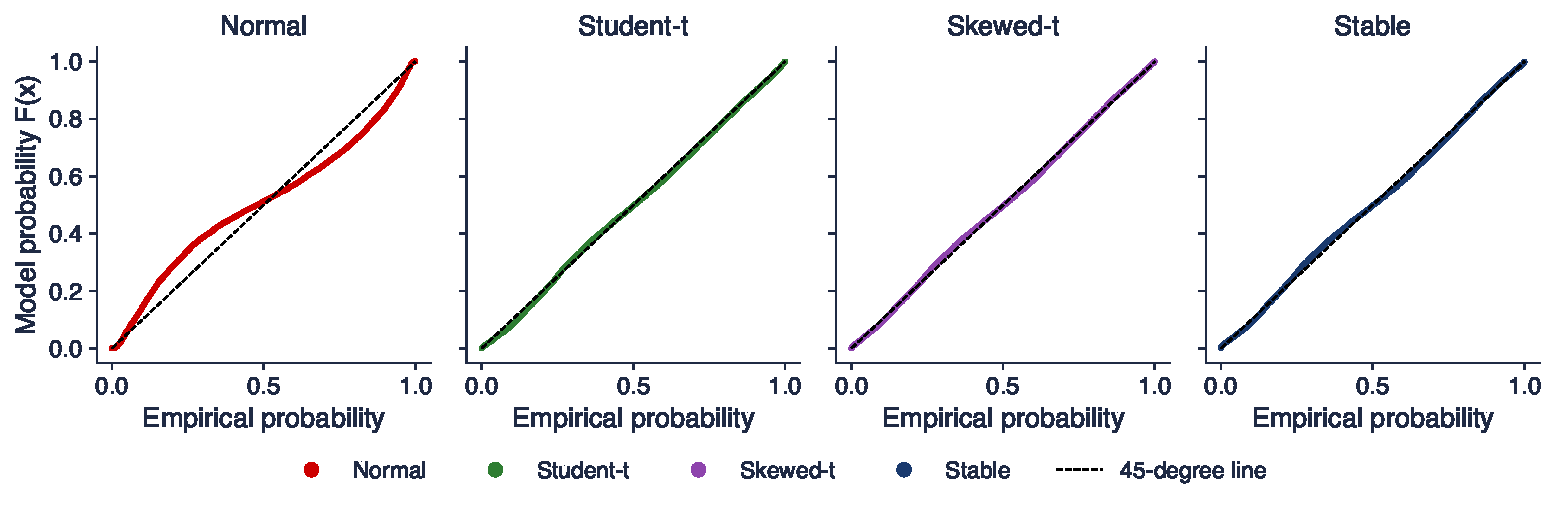
\includegraphics[width=0.97\textwidth,height=0.5\textheight,keepaspectratio]{sfm_ch6_pp.pdf}
\end{center}
\vspace{-0.25cm}
\begin{itemize}
    \item Normală: o formă de S în centru (prea puține randamente mici, prea multe de mărime medie), cea mai mare distanță $0{,}093$
    \item Student-t, skewed-t, stabilă: pe diagonală; într-un grafic PP nu se pot deosebi
\end{itemize}
\quantlet{SFM\_ch6\_pp\_qq}{\qlurl{SFM_ch6_pp_qq}}
\end{frame}

\begin{frame}{Grafice QQ: S\&P 500}
\itemsize{\footnotesize}
\begin{center}
    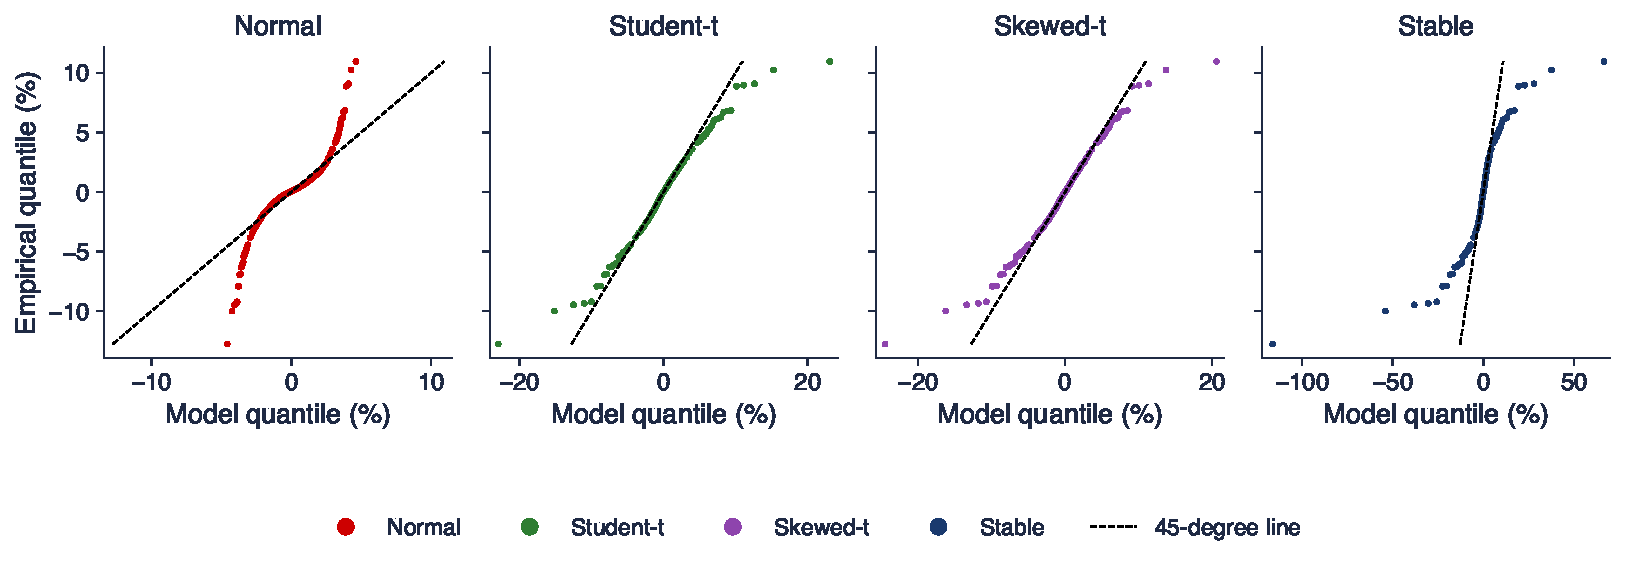
\includegraphics[width=0.97\textwidth,height=0.5\textheight,keepaspectratio]{sfm_ch6_qq.pdf}
\end{center}
\vspace{-0.25cm}
\begin{itemize}
    \item Cel mai mic randament zilnic a fost $-12{,}8\%$; cuantila modelului la aceeași probabilitate: Normală $-4{,}6\%$, Student-t $-22{,}9\%$, skewed-t $-24{,}5\%$, stabilă $-116{,}1\%$
    \item Modelele care păreau identice în graficul PP diferă puternic în extremitatea cozii
\end{itemize}
\quantlet{SFM\_ch6\_pp\_qq}{\qlurl{SFM_ch6_pp_qq}}
\end{frame}

\begin{frame}{Grafice QQ pentru BET, Bitcoin și Banca Transilvania}
\itemsize{\footnotesize}
\begin{center}
    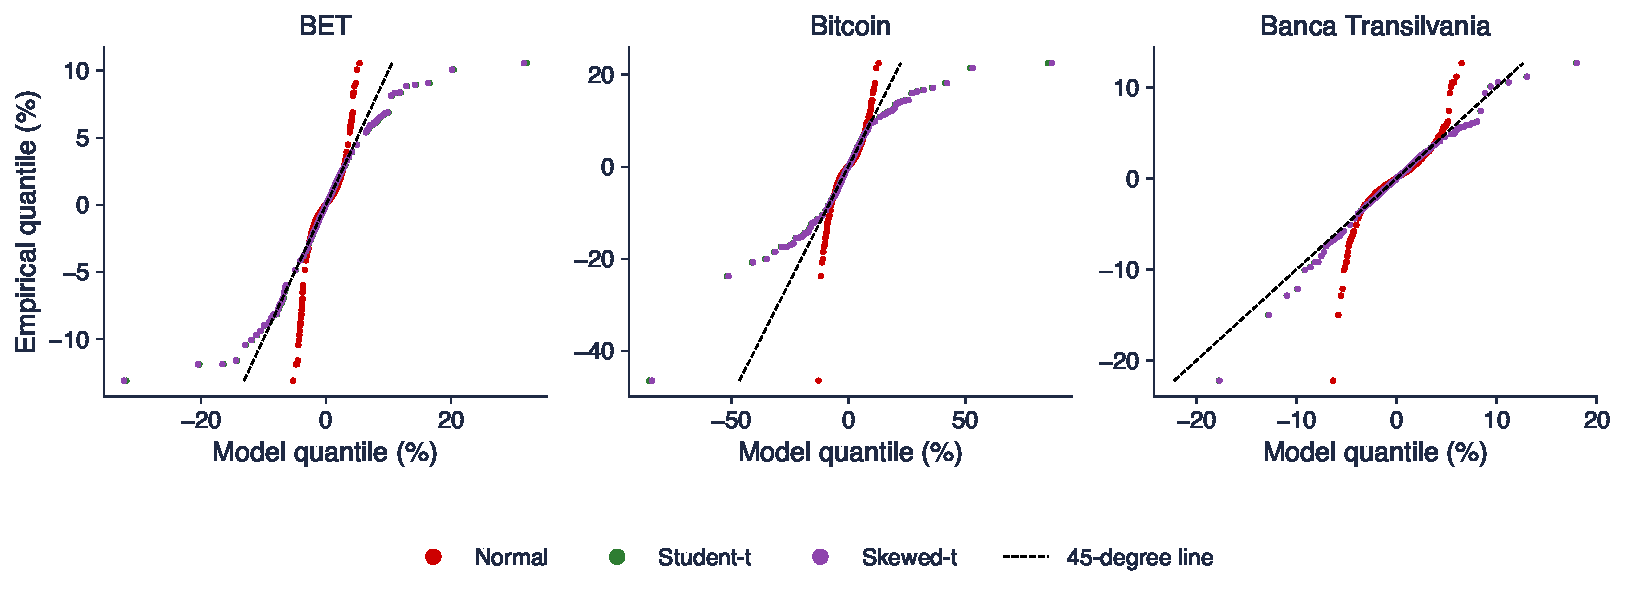
\includegraphics[width=0.97\textwidth,height=0.54\textheight,keepaspectratio]{sfm_ch6_qq_assets.pdf}
\end{center}
\vspace{-0.25cm}
\begin{itemize}
    \item Normală (roșu): capete abrupte pentru toate cele trei serii; Student-t și skewed-t urmăresc datele pînă departe în cozi
    \item Ultimele cîteva puncte sînt zile izolate (cele mai mari crahuri): acolo cozile estimate diferă cel mai mult, iar incertitudinea este cea mai mare
\end{itemize}
\quantlet{SFM\_ch6\_pp\_qq}{\qlurl{SFM_ch6_pp_qq}}
\end{frame}

\begin{frame}{Recapitulare: graficele PP și QQ}
\itemsize{\small}
\begin{itemize}
    \item PP: probabilități, util pentru centru; QQ: cuantile, util pentru cozi
    \item Modelele cu cozi groase care arată la fel în graficele PP diferă mult în graficele QQ
    \item Prezentați întotdeauna graficul QQ al modelului ales alături de valoarea AIC
\end{itemize}
\end{frame}


%=============================================================================
\section{Scopul decide: ce model estimează corect VaR 1\%?}
%=============================================================================

\begin{frame}{VaR și ES}
\itemsize{\small}
\begin{itemize}
    \item Randamentul $X$, nivelul $\alpha$ (aici $\alpha = 1\%$ sau $2{,}5\%$, probabilitatea cozii)
    \begin{itemize}
        \item \textbf{VaR} (Value at Risk, valoarea la risc): $\mathrm{VaR}_\alpha = -q_\alpha(X)$, pierderea depășită cu probabilitatea $\alpha$
        \item \textbf{ES} (expected shortfall, pierderea așteptată în coadă): $\mathrm{ES}_\alpha = -\frac{1}{\alpha}\int_0^\alpha q_u\, du = -E[X \mid X \le q_\alpha]$, pierderea medie din coadă
    \end{itemize}
    \item Modelul Normal: $\mathrm{VaR}_\alpha = -(\mu + \sigma z_\alpha)$, $z_{0{,}01} = -2{,}326$
    \begin{itemize}
        \item S\&P 500: $-(0{,}025 - 2{,}326 \times 1{,}213) = 2{,}80\%$, față de VaR 1\% empiric de $3{,}45\%$
    \end{itemize}
    \item Regulile Basel: ES 2,5\% pentru riscul de piață, VaR 1\% pentru backtesting (Capitolul 10)
\end{itemize}
\end{frame}

\begin{frame}{VaR 1\% și ES 2,5\% pentru fiecare model (în eșantion)}
\itemsize{\footnotesize}
\textbf{VaR 1\%} (\%)\begin{center}
\scriptsize
\begin{tabular}{lrrrrrrr}
\toprule
& date & Normală & Student-t & skewed-t & GED & NIG & stabilă \\
\midrule
BET & $4{,}13$ & $3{,}19$ & $4{,}06$ & $4{,}10$ & $3{,}74$ & $4{,}11$ & $4{,}94$ \\
S\&P 500 & $3{,}45$ & $2{,}80$ & $3{,}46$ & $3{,}71$ & $3{,}27$ & $3{,}72$ & $4{,}54$ \\
DAX & $4{,}16$ & $3{,}25$ & $3{,}96$ & $4{,}24$ & $3{,}77$ & $4{,}24$ & $5{,}01$ \\
Bitcoin & $10{,}51$ & $7{,}99$ & $11{,}06$ & $10{,}91$ & $9{,}85$ & $10{,}52$ & $14{,}26$ \\
TLV & $5{,}10$ & $4{,}01$ & $4{,}63$ & $4{,}61$ & $4{,}49$ & $4{,}76$ & $4{,}92$ \\
SNP & $4{,}29$ & $3{,}70$ & $4{,}26$ & $4{,}22$ & $4{,}16$ & $4{,}32$ & $4{,}43$ \\
BRD & $4{,}50$ & $3{,}81$ & $4{,}24$ & $4{,}39$ & $4{,}18$ & $4{,}43$ & $4{,}51$ \\
\bottomrule
\end{tabular}
\end{center}
\textbf{ES 2,5\%} (\%)\begin{center}
\scriptsize
\begin{tabular}{lrrrrrrr}
\toprule
& date & Normală & Student-t & skewed-t & GED & NIG & stabilă \\
\midrule
BET & $4{,}57$ & $3{,}21$ & $4{,}76$ & $4{,}81$ & $3{,}85$ & $4{,}31$ & $7{,}58$ \\
S\&P 500 & $3{,}76$ & $2{,}81$ & $3{,}95$ & $4{,}23$ & $3{,}36$ & $3{,}89$ & $6{,}70$ \\
Bitcoin & $10{,}84$ & $8{,}03$ & $13{,}37$ & $13{,}18$ & $10{,}17$ & $11{,}06$ & $22{,}87$ \\
\bottomrule
\end{tabular}
\end{center}
\quantlet{SFM\_ch6\_tail\_var}{\qlurl{SFM_ch6_tail_var}}
\end{frame}

\begin{frame}{VaR 1\% al modelelor raportat la date}
\itemsize{\footnotesize}
\begin{center}
    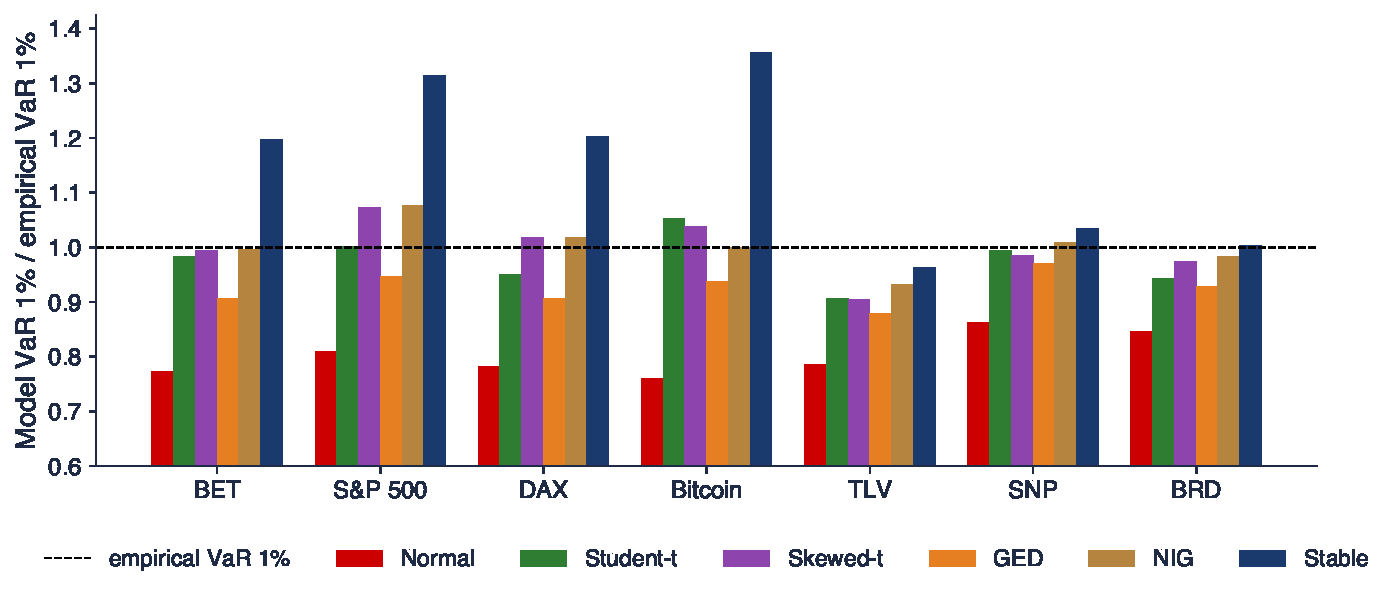
\includegraphics[width=0.97\textwidth,height=0.55\textheight,keepaspectratio]{sfm_ch6_var_models.pdf}
\end{center}
\vspace{-0.25cm}
\begin{itemize}
    \item Normală: prea mic cu $14$--$24\%$ pe toate seriile; stabilă: prea mare cu pînă la $36\%$
    \item Student-t, skewed-t și NIG se abat cu cel mult $10\%$ de la VaR 1\% empiric; GED este puțin prea mic
\end{itemize}
\quantlet{SFM\_ch6\_tail\_var}{\qlurl{SFM_ch6_tail_var}}
\end{frame}

\begin{frame}{Coada stîngă pe axe log-log (S\&P 500)}
\itemsize{\footnotesize}
\begin{center}
    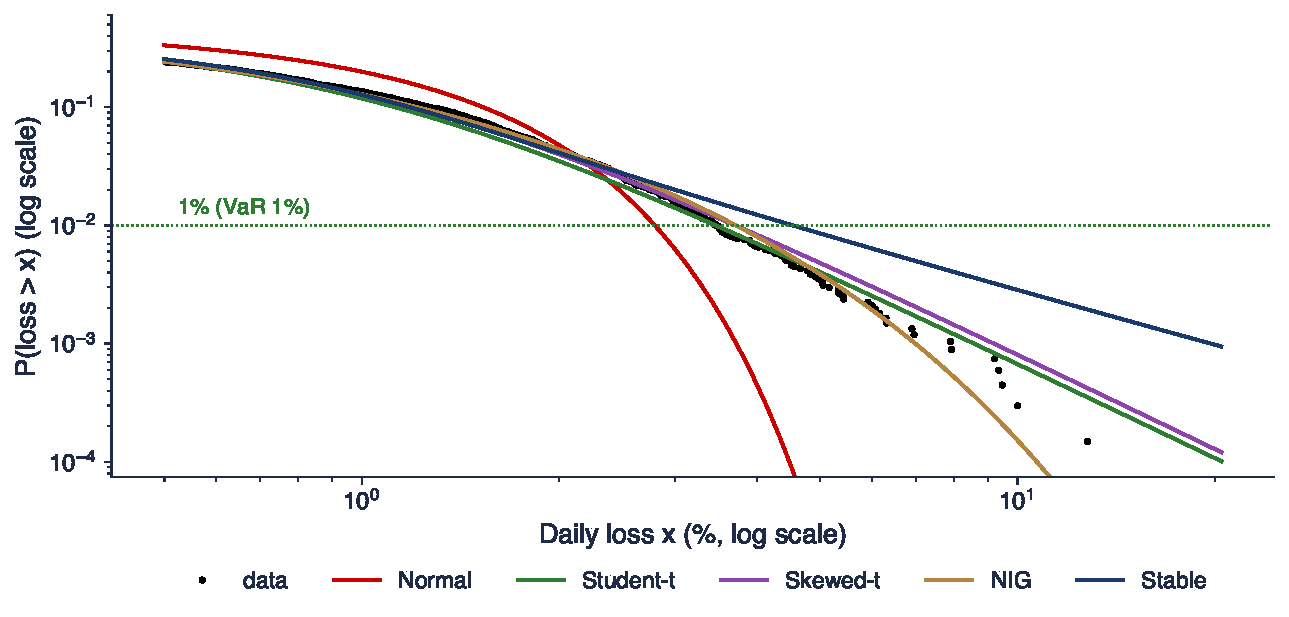
\includegraphics[width=0.97\textwidth,height=0.58\textheight,keepaspectratio]{sfm_ch6_left_tail.pdf}
\end{center}
\vspace{-0.25cm}
\begin{itemize}
    \item Punctele: proporția zilelor cu o pierdere peste $x$; liniile: aceeași probabilitate pentru fiecare model estimat
    \item La 1\%, toate modelele cu cozi groase sînt apropiate; pentru pierderi de peste $5\%$, curba distribuției stabile este mult prea sus, iar cea Normală scade abrupt
\end{itemize}
\quantlet{SFM\_ch6\_tail\_var}{\qlurl{SFM_ch6_tail_var}}
\end{frame}

\begin{frame}{Numărarea depășirilor: testul Kupiec}
\itemsize{\footnotesize}
\begin{center}
\scriptsize
\begin{tabular}{lrrrrrrr}
\toprule
& așteptat & Normală & Student-t & skewed-t & GED & NIG & stabilă \\
\midrule
BET & 67 & 138 & 71 & 69 & 91 & 68 & 43 \\
S\&P 500 & 67 & 131 & 67 & 52 & 80 & 52 & 30 \\
DAX & 68 & 145 & 78 & 66 & 91 & 65 & 39 \\
Bitcoin & 44 & 86 & 34 & 36 & 56 & 44 & 16 \\
\bottomrule
\end{tabular}
\end{center}
\begin{itemize}
    \item Depășire: o zi cu $r_t < -\mathrm{VaR}_{1\%}$; pentru un model corect, numărul lor este $\mathrm{Binomial}(n; 0{,}01)$
    \item \refKupiec: $LR_{uc} = -2\ln\dfrac{(1-\alpha)^{n - x}\alpha^x}{(1 - x/n)^{n - x}(x/n)^x} \approx \chi^2(1)$, $x$ = numărul de depășiri
    \item S\&P 500: Student-t, 67 depășiri față de 67 așteptate ($p = 0{,}986$); NIG, cîștigătorul AIC, 52 ($p = 0{,}053$)
    \item Cel mai bun model pentru întreaga densitate nu este întotdeauna cel mai bun pentru o cuantilă; există scoruri axate pe coadă \refDPD
\end{itemize}\quantlet{SFM\_ch6\_tail\_var}{\qlurl{SFM_ch6_tail_var}}
\end{frame}

\begin{frame}{Recapitulare: VaR 1\% în eșantion}
\itemsize{\small}
\begin{itemize}
    \item VaR 1\% $= -q_{1\%}$, ES 2,5\% = pierderea medie dincolo de $q_{2{,}5\%}$
    \item Normală: VaR 1\% cu $14$--$24\%$ prea mic; stabilă: mult prea mare; Student-t, skewed-t, NIG: apropiate
    \item Judecați un model de risc după depășirile lui (Kupiec), nu doar după AIC
\end{itemize}
\end{frame}


%=============================================================================
\section{În afara eșantionului: validare și supraajustare}
%=============================================================================

\begin{frame}{De ce în afara eșantionului?}
\itemsize{\small}
\begin{itemize}
    \item În eșantion, un model mai general se ajustează cel puțin la fel de bine: $\ell$ nu scade niciodată cînd adăugăm parametri
    \begin{itemize}
        \item \textbf{supraajustare} (overfitting): parametrii suplimentari modelează zgomotul eșantionului de estimare, nu trăsături ale randamentelor viitoare
    \end{itemize}
    \item Verificarea onestă: estimăm pînă la 31 decembrie 2019 și evaluăm pe 2020--2026 (crahul COVID-19, șocul inflației din 2022, taxele vamale din 2025)
    \begin{itemize}
        \item \textbf{scorul logaritmic}: media lui $\ln f(r_t; \hat\theta)$ pe zilele de test; valoarea mai mare este preferată; este o regulă de scor proprie (proper scoring rule) \refGR
        \item \textbf{depășirile} VaR 1\% (Kupiec) și \textbf{pierderea pinball} $\frac{1}{n}\sum_t (\alpha - \mathbf{1}\{r_t < q\})(r_t - q)$ a cuantilei de 1\% $q$
    \end{itemize}
    \item Un scor este \textbf{propriu} dacă distribuția adevărată obține cel mai bun scor așteptat: prognozistul nu are nimic de cîștigat dacă își distorsionează prognoza
\end{itemize}
\end{frame}

\begin{frame}{Rezultate în afara eșantionului, 2020--2026}
\itemsize{\footnotesize}
\begin{center}
    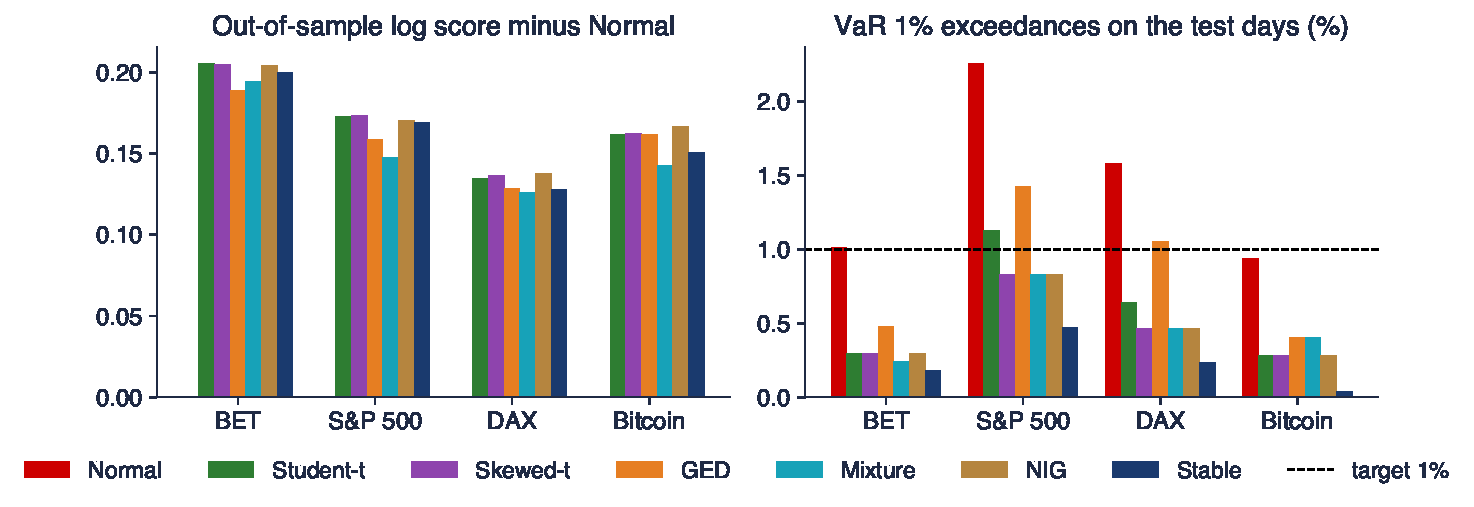
\includegraphics[width=0.97\textwidth,height=0.55\textheight,keepaspectratio]{sfm_ch6_oos.pdf}
\end{center}
\vspace{-0.25cm}
\begin{itemize}
    \item Stînga: fiecare model cu cozi groase depășește scorul logaritmic al modelului Normal cu $0{,}13$ pînă la $0{,}21$ pe zi; diferențele dintre ele sînt mici
    \item Dreapta: ratele de depășire ale VaR 1\%; ținta este linia punctată de la 1\%
\end{itemize}
\quantlet{SFM\_ch6\_out\_of\_sample}{\qlurl{SFM_ch6_out_of_sample}}
\end{frame}

\begin{frame}{Interpretarea tabelului din afara eșantionului}
\itemsize{\footnotesize}
\begin{center}
\scriptsize
\begin{tabular}{lrrrrrrrll}
\toprule
& aștept. & Normală & t & skew-t & NIG & stabilă & ist. & cel mai bun AIC & cel mai bun scor \\
\midrule
BET & 16{,}7 & 17 & 5 & 5 & 5 & 3 & 5 & NIG & Student-t \\
S\&P 500 & 16{,}9 & 38 & 19 & 14 & 14 & 8 & 23 & NIG & skewed-t \\
DAX & 17{,}1 & 27 & 11 & 8 & 8 & 4 & 8 & NIG & NIG \\
Bitcoin & 24{,}5 & 23 & 7 & 7 & 7 & 1 & 10 & GED & NIG \\
\bottomrule
\end{tabular}
\end{center}
\begin{itemize}
    \item Depășiri ale VaR 1\% pe zilele de test; aștept.: numărul așteptat; ist.: simularea istorică (cuantila de 1\% a eșantionului de estimare)
    \item Cîștigătorul AIC din 2000--2019 are cel mai bun scor logaritmic doar pentru DAX; în rest, cel mai bun scor aparține unui model apropiat în clasament
    \item BET: modelul Normal are 17 depășiri față de 16{,}7 așteptate, modelele cu cozi groase doar 5: perioada 2020--2026 a fost mai calmă pentru BET decît 2000--2019
    \item Numărul potrivit, dar din motive greșite: un model static nu poate urmări schimbările de volatilitate
\end{itemize}\quantlet{SFM\_ch6\_out\_of\_sample}{\qlurl{SFM_ch6_out_of_sample}}
\end{frame}

\begin{frame}{Supraajustare: amestecuri Normale cu 1 pînă la 6 componente}
\itemsize{\footnotesize}
\begin{center}
    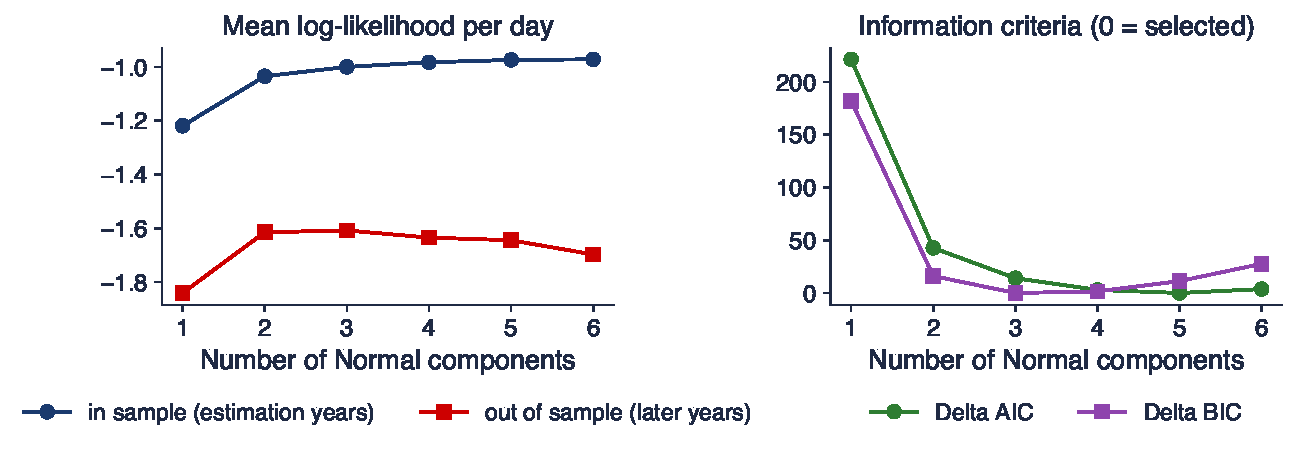
\includegraphics[width=0.97\textwidth,height=0.52\textheight,keepaspectratio]{sfm_ch6_overfit.pdf}
\end{center}
\vspace{-0.25cm}
\begin{itemize}
    \item S\&P 500, estimare 2017--2018 ($n = 501$), test 2019--2026 ($n = 1\,939$); $c$ componente au $3c - 1$ parametri
    \item În eșantion (albastru), calitatea ajustării crește cu fiecare componentă; în afara eșantionului (roșu) atinge maximul la $c = 3$ și apoi scade
\end{itemize}
\quantlet{SFM\_ch6\_out\_of\_sample}{\qlurl{SFM_ch6_out_of_sample}}
\end{frame}

\begin{frame}{Care criteriu ne-a avertizat?}
\itemsize{\small}
\begin{itemize}
    \item Log-verosimilitatea medie pe zi, în eșantion $\to$ în afara eșantionului
    \begin{itemize}
        \item $c = 1$ (Normală): $-1{,}219 \to -1{,}841$; $c = 3$: $-0{,}999 \to -1{,}608$; $c = 6$ (17 parametri): $-0{,}971 \to -1{,}698$
    \end{itemize}
    \item BIC a ales $c = 3$, cel mai bun model în afara eșantionului; AIC a ales $c = 5$
    \begin{itemize}
        \item cu $n = 501$, penalizarea AIC de 2 pe parametru este prea slabă pentru a opri componentele în plus
    \end{itemize}
    \item Diferența dintre ajustarea în eșantion și cea din afara lui crește cu numărul de parametri: această diferență este supraajustarea
    \item Regula: eșantioane scurte, mulți parametri $\Rightarrow$ preferați BIC sau AICc și păstrați întotdeauna o perioadă de test
\end{itemize}\quantlet{SFM\_ch6\_out\_of\_sample}{\qlurl{SFM_ch6_out_of_sample}}
\end{frame}

\begin{frame}{VaR 1\% pe fereastră mobilă: reestimare lunară}
\itemsize{\footnotesize}
\begin{center}
    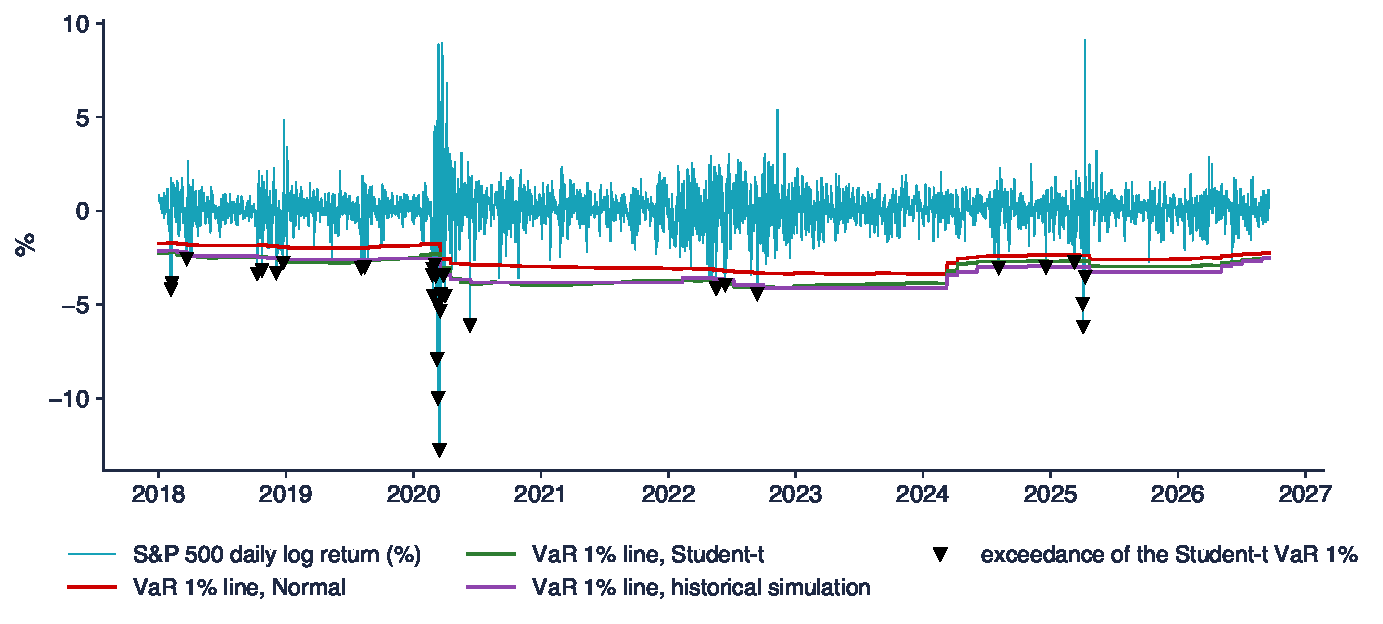
\includegraphics[width=0.97\textwidth,height=0.55\textheight,keepaspectratio]{sfm_ch6_rolling_var.pdf}
\end{center}
\vspace{-0.25cm}
\begin{itemize}
    \item S\&P 500: fiecare model este reestimat la fiecare 20 de zile de tranzacționare pe cele 1000 de zile anterioare; linia VaR 1\% este desenată ca prag de pierdere $-\mathrm{VaR}$
    \item Triunghiurile negre: depășiri ale VaR Student-t; apar grupat (martie 2020)
\end{itemize}
\quantlet{SFM\_ch6\_out\_of\_sample}{\qlurl{SFM_ch6_out_of_sample}}
\end{frame}

\begin{frame}{Backtesting pe fereastră mobilă: rezultatele}
\itemsize{\footnotesize}
\begin{center}
\footnotesize
\begin{tabular}{lrrrr}
\toprule
& Normală & Student-t & skewed-t & istorică \\
\midrule
S\&P 500, rata (\%) & $2{,}35$ & $1{,}56$ & $1{,}47$ & $1{,}58$ \\
S\&P 500, Kupiec $p$ & $<0{,}001$ & $<0{,}001$ & $<0{,}001$ & $<0{,}001$ \\
S\&P 500, maximul anual & 36 & 31 & 28 & 29 \\
BET, rata (\%) & $1{,}98$ & $1{,}52$ & $1{,}38$ & $1{,}25$ \\
BET, Kupiec $p$ & $<0{,}001$ & $<0{,}001$ & $0{,}007$ & $0{,}066$ \\
\bottomrule
\end{tabular}
\end{center}
\begin{itemize}
    \item Backtesting 2003--2026, $n = 5\,714$ zile pentru S\&P 500; rata țintă 1\%; cel mai slab an este 2008, pentru toate modelele și pentru ambele serii
    \item Cozile groase înjumătățesc excesul de depășiri, dar niciun model necondiționat nu ajunge la 1\%: volatilitatea se schimbă mai repede decît se poate adapta o fereastră de 1000 de zile
    \item Remediul este un model pentru volatilitatea însăși: GARCH, \sfmchlink{https://danpele.github.io/SFM/RO/Cursuri/capitol8_estimatori_volatilitate.pdf}{Capitolele 8} și \sfmchlink{https://danpele.github.io/SFM/RO/Cursuri/capitol9_modele_arch_garch.pdf}{9}
\end{itemize}\quantlet{SFM\_ch6\_out\_of\_sample}{\qlurl{SFM_ch6_out_of_sample}}
\end{frame}

\begin{frame}{Graficul de fiabilitate VaR (SFEVaRqqplot)}
\itemsize{\footnotesize}
\begin{center}
    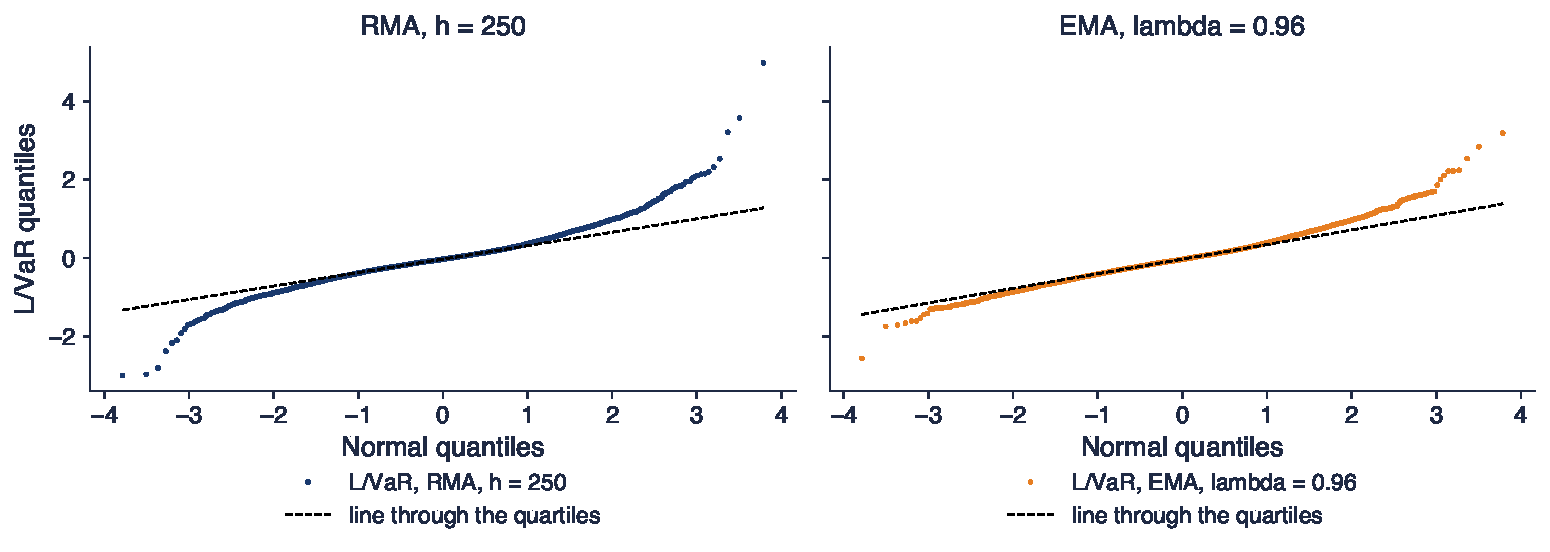
\includegraphics[width=0.97\textwidth,height=0.52\textheight,keepaspectratio]{sfm_ch6_var_qqplot.pdf}
\end{center}
\vspace{-0.25cm}
\begin{itemize}
    \item DAX din 2000: VaR 1\% Normal cu volatilitatea ultimelor 250 de zile, RMA (rectangular moving average, medie mobilă simplă) sau EMA (exponential moving average, medie mobilă exponențială, $\lambda = 0{,}96$); graficul QQ al lui $L/\mathrm{VaR}$ față de cuantilele Normale
    \item O dreaptă ar însemna un VaR fiabil; ambele se curbează în sus la capătul drept: pierderile dincolo de VaR sînt prea mari și prea frecvente ($2{,}13\%$ și $2{,}07\%$ depășiri)
\end{itemize}
\quantlet{SFM\_ch6\_var\_qqplot}{\qlurl{SFM_ch6_var_qqplot}}
\end{frame}

\begin{frame}{Recapitulare: în afara eșantionului}
\itemsize{\small}
\begin{itemize}
    \item Judecați modelele pe date pe care nu le-au văzut: scor logaritmic, depășiri, pierdere pinball
    \item Supraajustarea: calitatea ajustării în eșantion crește cu numărul de parametri, cea din afara lui nu; BIC ne-a protejat, AIC nu
    \item Cozile groase ajută, dar modelele statice eșuează în crize: volatilitatea trebuie modelată (GARCH)
\end{itemize}
\end{frame}


%=============================================================================
\section{Incertitudinea de model}
%=============================================================================

\begin{frame}{Cît de siguri sîntem de cîștigător?}
\itemsize{\footnotesize}
\begin{center}
    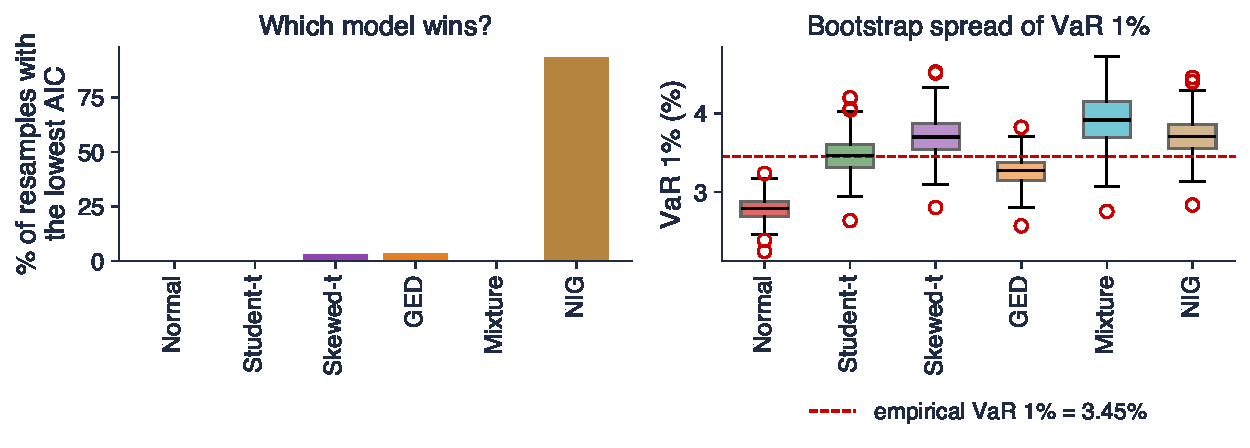
\includegraphics[width=0.97\textwidth,height=0.52\textheight,keepaspectratio]{sfm_ch6_model_uncertainty.pdf}
\end{center}
\vspace{-0.25cm}
\begin{itemize}
    \item S\&P 500, 200 de reeșantionări bootstrap pe blocuri mobile (blocurile de 20 de zile păstrează volatility clustering); în fiecare reeșantionare, cele șase modele sînt reestimate
    \item Stînga: NIG are cel mai mic AIC în $94\%$ din reeșantionări; dreapta: dispersia bootstrap a VaR 1\% pentru fiecare model
\end{itemize}
\quantlet{SFM\_ch6\_model\_uncertainty}{\qlurl{SFM_ch6_model_uncertainty}}
\end{frame}

\begin{frame}{Două surse de incertitudine}
\itemsize{\small}
\begin{itemize}
    \item \textbf{Incertitudinea parametrilor}: același model, reestimat pe date reeșantionate
    \begin{itemize}
        \item VaR 1\% Student-t: intervalul bootstrap de 90\% $[3{,}14; 3{,}87]\%$; NIG: $[3{,}34; 4{,}18]\%$
    \end{itemize}
    \item \textbf{Incertitudinea de model}: modele diferite pe aceleași date
    \begin{itemize}
        \item VaR 1\% median: GED $3{,}27\%$, Student-t $3{,}47\%$, NIG $3{,}71\%$, amestec Normal $3{,}92\%$
        \item dispersia dintre modele este comparabilă cu dispersia din interiorul unui model
    \end{itemize}
    \item Chiar cînd cîștigătorul AIC este clar, cifra relevantă pentru risc rămîne incertă
    \item Măsurile de coadă construite pe baza entropiei oferă o altă cale de a rezuma această incertitudine: \refPeleA, \refPeleB
\end{itemize}
\end{frame}

\begin{frame}{Medierea modelelor și riscul de model}
\itemsize{\footnotesize}
\begin{center}
\scriptsize
\begin{tabular}{lrrrrr}
\toprule
& date & Normală & interval (cozi groase) & mediat & interval (\%) \\
\midrule
BET & $4{,}13$ & $3{,}19$ & $[3{,}74; 4{,}94]$ & $4{,}11$ & $32$ \\
S\&P 500 & $3{,}45$ & $2{,}80$ & $[3{,}27; 4{,}54]$ & $3{,}72$ & $39$ \\
DAX & $4{,}16$ & $3{,}25$ & $[3{,}77; 5{,}01]$ & $4{,}24$ & $33$ \\
Bitcoin & $10{,}51$ & $7{,}99$ & $[9{,}85; 14{,}26]$ & $9{,}85$ & $45$ \\
TLV & $5{,}10$ & $4{,}01$ & $[4{,}49; 5{,}41]$ & $4{,}62$ & $21$ \\
SNP & $4{,}29$ & $3{,}70$ & $[4{,}16; 4{,}70]$ & $4{,}25$ & $13$ \\
BRD & $4{,}50$ & $3{,}81$ & $[4{,}18; 4{,}74]$ & $4{,}33$ & $14$ \\
\bottomrule
\end{tabular}
\end{center}
\begin{itemize}
    \item VaR 1\% în \%; intervalul cozilor groase: cel mai mic și cel mai mare VaR 1\% dintre cele șase modele nenormale; intervalul (\%): max/min $- 1$
    \item Mediat: $\sum_i w_i\,\mathrm{VaR}_i$ cu ponderile Akaike; un analog frecventist al medierii bayesiene a modelelor \refHoeting
    \item \textbf{Riscul de model}: amplitudinea rezultatelor între modelele plauzibile; autoritățile de supraveghere cer băncilor să îl măsoare \refKerkhof, \refDanielsson
\end{itemize}\quantlet{SFM\_ch6\_model\_uncertainty}{\qlurl{SFM_ch6_model_uncertainty}}
\end{frame}

\begin{frame}{Etapele selecției modelului}
\itemsize{\small}
\begin{itemize}
    \item \textbf{1. Datele}: comparați cele mai mari randamente cu prețurile și cu știrile; eliminați doar erorile dovedite
    \item \textbf{2. Candidații}: alegeți-i după faptele stilizate (cozi, asimetrie), nu după comoditate
    \item \textbf{3. Ajustare și clasament}: ML, apoi AIC și BIC; teste LR pentru perechile imbricate, Vuong pentru celelalte
    \item \textbf{4. Verificare}: statistica AD și graficul QQ pentru primele modele din clasament; modelul trebuie să se potrivească bine în zona care vă interesează
    \item \textbf{5. Validare}: în afara eșantionului, cu funcția de pierdere potrivită scopului (depășiri pentru VaR)
    \item \textbf{6. Raportare}: cîștigătorul, modelele de pe locurile următoare și intervalul valorilor de risc între acestea
\end{itemize}
\end{frame}

\begin{frame}{Recapitulare: incertitudinea de model}
\itemsize{\small}
\begin{itemize}
    \item Cîștigătorul AIC poate fi stabil între reeșantionări, în timp ce VaR nu este
    \item Raportați intervalul dintre modelele plauzibile sau mediați cu ponderile Akaike
    \item Riscul de model face parte din risc: o singură cifră îl ascunde
\end{itemize}
\end{frame}


%=============================================================================
\section{AI pentru descoperire științifică}
%=============================================================================

\begin{frame}{O întrebare deschisă}
\itemsize{\small}
\begin{itemize}
    \item \textbf{Mai cîștigă NIG după ce eliminăm efectul de volatility clustering?}
    \begin{itemize}
        \item o parte din cozile groase ale randamentelor zilnice provine din volatilitatea variabilă în timp (\sfmchlink{https://danpele.github.io/SFM/RO/Cursuri/capitol2_distributii_clasice_fapte_stilizate.pdf}{Capitolul 2})
        \item randamentele împărțite la o prognoză de volatilitate (de exemplu EMA, $\lambda = 0{,}96$) au cozi mai subțiri; care candidat li se potrivește cel mai bine?
    \end{itemize}
    \item De ce este deschisă: răspunsul diferă de la o piață la alta, iar modelul de volatilitate este el însuși o alegere
    \item Randamentele zilnice brute: NIG cîștigă pentru cei trei indici, GED pentru Bitcoin, Student-t pentru acțiunile BVB (acest capitol)
    \item Instrumentele AI pot accelera un astfel de studiu; nu înlocuiesc verificarea lui \refWang
\end{itemize}
\end{frame}

\begin{frame}{Contribuția posibilă a AI}
\itemsize{\small}
\begin{itemize}
    \item \textbf{Literatura}: lista studiilor care compară distribuțiile randamentelor după filtrarea GARCH, cu eșantioanele și criteriile lor
    \item \textbf{Cod}: o primă versiune a buclei „standardizează, ajustează șapte modele, ordonează după AIC și BIC, testează în afara eșantionului”
    \item \textbf{Robustețe}: alte filtre de volatilitate, alte ferestre și alte piețe
    \item \textbf{Explicație}: o primă explicație a schimbării clasamentului după filtrare
    \item Exemplu de prompt
    \begin{itemize}
        \item \aiprompt{Write Python code that divides daily log returns by an EMA volatility (lambda = 0.96), fits Normal, Student-t, skewed-t, GED and NIG by maximum likelihood, and reports AIC, BIC and Akaike weights.}
    \end{itemize}
\end{itemize}
\end{frame}

\begin{frame}{Verificări necesare}
\itemsize{\small}
\begin{itemize}
    \item Informația din viitor (look-ahead bias): volatilitatea zilei $t$ trebuie să folosească doar randamentele pînă la $t - 1$
    \item Numărul de parametri: $k$ din AIC trebuie să includă fiecare parametru estimat, inclusiv pe cei ai filtrului de volatilitate, dacă au fost estimați
    \item Aceleași date pentru toate modelele: valorile AIC calculate pe eșantioane diferite nu se pot compara
    \item Parametrizările: scală sau abatere standard la Student-t; S0 sau S1 la distribuția stabilă
    \item Referințele: fiecare lucrare citată trebuie să existe; verificați DOI-ul
\end{itemize}
\end{frame}

\begin{frame}{Idee de proiect}
\itemsize{\small}
\begin{itemize}
    \item \textbf{Întrebarea}: diferă cea mai bună distribuție pentru randamentele standardizate de cea pentru randamentele brute?
    \begin{itemize}
        \item date: BET, S\&P 500, DAX, Bitcoin și acțiunile BVB din datele cursului (EODHD)
    \end{itemize}
    \item Pași
    \begin{itemize}
        \item standardizați cu volatilitatea EMA; ajustați cei șapte candidați; tabel cu $\Delta$AIC și ponderile Akaike
        \item repetați backtesting-ul VaR 1\% în afara eșantionului din acest capitol cu modelul standardizat
        \item comparați grupurile de depășiri din 2008 și 2020 cu cele ale modelelor necondiționate
    \end{itemize}
    \item Rezultat: un tabel, un grafic și un paragraf despre ce se schimbă și de ce
    \item Declarați orice folosire a AI și enumerați erorile AI pe care le-ați corectat
\end{itemize}
\end{frame}


%=============================================================================
\section{Rezumat}
%=============================================================================

\begin{frame}{Idei de reținut}
\itemsize{\small}
\begin{itemize}
    \item Alegerea modelului începe cu date curate și un scop: corpul sau coada?
    \item ML estimează parametrii; testele LR compară modele imbricate (atenție la frontiere); Vuong le compară pe cele neimbricate
    \item AIC și BIC ordonează toți candidații; citiți $\Delta$ și ponderile Akaike
    \item Testele EDF: AD pune accentul pe cozi, KS nu; cu $n$ mare toate modelele sînt respinse, deci ordonați modelele și examinați graficele
    \item Pe randamentele reale cîștigă NIG, GED și Student-t; distribuțiile Normală și stabilă pierd peste tot
    \item Validați în afara eșantionului și raportați intervalul VaR între modelele plauzibile
\end{itemize}
\end{frame}

\begin{frame}{Formule de reținut}
\itemsize{\small}
{\renewcommand{\arraystretch}{1.4}\begin{center}
\scriptsize
\begin{tabular}{ll}
\toprule
\textbf{Mărimea} & \textbf{Formula} \\
\midrule
Log-verosimilitatea & $\ell(\theta) = \sum_t \ln f(r_t; \theta)$ \\
Raportul de verosimilitate & $LR = 2(\ell_1 - \ell_0) \approx \chi^2(k_1 - k_0)$ \\
AIC, BIC & $-2\ell(\hat\theta) + 2k$, \quad $-2\ell(\hat\theta) + k\ln n$ \\
Ponderea Akaike & $w_i = e^{-\Delta_i/2} / \sum_j e^{-\Delta_j/2}$ \\
Vuong & $V = \sqrt{n}\,\bar m / s_m$, \quad $m_t = \ln f_1(r_t) - \ln f_2(r_t)$ \\
KS & $D_n = \sup_x |F_n(x) - F(x)|$ \\
Anderson--Darling & $A^2 = n\int [F_n - F]^2 / [F(1 - F)]\, dF$ \\
Kupiec & $LR_{uc} = -2\ln\frac{(1-\alpha)^{n - x}\alpha^x}{(1 - x/n)^{n - x}(x/n)^x}$ \\
Pierderea pinball & $\frac{1}{n}\sum_t (\alpha - \mathbf{1}\{r_t < q\})(r_t - q)$ \\
\bottomrule
\end{tabular}
\end{center}
}
\end{frame}

\begin{frame}{Autoevaluare}
\itemsize{\small}
\begin{itemize}
    \item \textbf{Întrebare}: modelul A are $\ell = -1000$ cu $k = 3$, modelul B are $\ell = -998$ cu $k = 5$; care are AIC mai mic?
    \begin{itemize}
        \item \textbf{Răspuns}: A: $2006$; B: $2006$; egalitate ($\Delta = 0$): cei doi parametri în plus aduc un cîștig egal exact cu penalizarea lor
    \end{itemize}
    \item \textbf{Întrebare}: A este imbricat în B; este B semnificativ mai bun la 5\%?
    \begin{itemize}
        \item \textbf{Răspuns}: $LR = 2 \cdot 2 = 4 < \chi^2_{0{,}95}(2) = 5{,}99$: nu
    \end{itemize}
    \item \textbf{Întrebare}: de ce nu poate un test KS cu parametri estimați să folosească tabelul KS clasic?
    \begin{itemize}
        \item \textbf{Răspuns}: estimarea apropie $F$ de date, deci $D_n$ este prea mic; folosiți Lilliefors sau un bootstrap parametric
    \end{itemize}
    \item Urmează: \sfmchlink{https://danpele.github.io/SFM/RO/Cursuri/capitol7_piete_eficiente_mers_aleator_vr.pdf}{Capitolul 7}, piețele eficiente, mersul aleator și testele variance ratio
\end{itemize}
\end{frame}


%=============================================================================
\section{Bibliografie}
%=============================================================================

\begin{frame}{Bibliografie (1/3)}
\itemsize{\tiny}
\begin{itemize}
    \item Akaike, H. (1974). \href{https://doi.org/10.1109/TAC.1974.1100705}{A new look at the statistical model identification}. \textit{IEEE Transactions on Automatic Control}, 19(6), 716--723.
    \item Amisano, G., Giacomini, R. (2007). \href{https://doi.org/10.1198/073500106000000332}{Comparing density forecasts via weighted likelihood ratio tests}. \textit{Journal of Business \& Economic Statistics}, 25(2), 177--190.
    \item Anderson, T.W., Darling, D.A. (1952). \href{https://doi.org/10.1214/aoms/1177729437}{Asymptotic theory of certain ``goodness of fit'' criteria based on stochastic processes}. \textit{Annals of Mathematical Statistics}, 23(2), 193--212.
    \item Anderson, T.W., Darling, D.A. (1954). \href{https://doi.org/10.1080/01621459.1954.10501232}{A test of goodness of fit}. \textit{Journal of the American Statistical Association}, 49(268), 765--769.
    \item Barndorff-Nielsen, O.E. (1997). \href{https://doi.org/10.1111/1467-9469.00045}{Normal inverse Gaussian distributions and stochastic volatility modelling}. \textit{Scandinavian Journal of Statistics}, 24(1), 1--13.
    \item Borak, S., Härdle, W.K., López-Cabrera, B. (2013). \href{https://doi.org/10.1007/978-3-642-33929-5}{\textit{Statistics of Financial Markets: Exercises and Solutions}}, 2nd ed. Springer.
    \item Box, G.E.P. (1976). \href{https://doi.org/10.1080/01621459.1976.10480949}{Science and statistics}. \textit{Journal of the American Statistical Association}, 71(356), 791--799.
    \item Burnham, K.P., Anderson, D.R. (2002). \href{https://doi.org/10.1007/b97636}{\textit{Model Selection and Multimodel Inference: A Practical Information-Theoretic Approach}}, 2nd ed. Springer.
    \item Burnham, K.P., Anderson, D.R. (2004). \href{https://doi.org/10.1177/0049124104268644}{Multimodel inference: understanding AIC and BIC in model selection}. \textit{Sociological Methods \& Research}, 33(2), 261--304.
    \item Cont, R. (2001). \href{https://doi.org/10.1080/713665670}{Empirical properties of asset returns: stylized facts and statistical issues}. \textit{Quantitative Finance}, 1(2), 223--236.
    \item Cramér, H. (1928). \href{https://doi.org/10.1080/03461238.1928.10416862}{On the composition of elementary errors}. \textit{Scandinavian Actuarial Journal}, 1928(1), 13--74.
    \item Danielsson, J., James, K.R., Valenzuela, M., Zer, I. (2016). \href{https://doi.org/10.1016/j.jfs.2016.02.002}{Model risk of risk models}. \textit{Journal of Financial Stability}, 23, 79--91.
    \item Diks, C., Panchenko, V., van Dijk, D. (2011). \href{https://doi.org/10.1016/j.jeconom.2011.04.001}{Likelihood-based scoring rules for comparing density forecasts in tails}. \textit{Journal of Econometrics}, 163(2), 215--230.
    \item Eberlein, E., Keller, U. (1995). \href{https://doi.org/10.2307/3318481}{Hyperbolic distributions in finance}. \textit{Bernoulli}, 1(3), 281--299.
    \item Franke, J., Härdle, W.K., Hafner, C.M. (2019). \href{https://doi.org/10.1007/978-3-030-13751-9}{\textit{Statistics of Financial Markets: An Introduction}}, 5th ed. Springer.
    \item Gneiting, T., Raftery, A.E. (2007). \href{https://doi.org/10.1198/016214506000001437}{Strictly proper scoring rules, prediction, and estimation}. \textit{Journal of the American Statistical Association}, 102(477), 359--378.
\end{itemize}
\end{frame}

\begin{frame}{Bibliografie (2/3)}
\itemsize{\tiny}
\begin{itemize}
    \item Hansen, B.E. (1994). \href{https://doi.org/10.2307/2527081}{Autoregressive conditional density estimation}. \textit{International Economic Review}, 35(3), 705--730.
    \item Hoeting, J.A., Madigan, D., Raftery, A.E., Volinsky, C.T. (1999). \href{https://doi.org/10.1214/ss/1009212519}{Bayesian model averaging: a tutorial}. \textit{Statistical Science}, 14(4), 382--417.
    \item Hurvich, C.M., Tsai, C.-L. (1989). \href{https://doi.org/10.1093/biomet/76.2.297}{Regression and time series model selection in small samples}. \textit{Biometrika}, 76(2), 297--307.
    \item Kerkhof, J., Melenberg, B., Schumacher, H. (2010). \href{https://doi.org/10.1016/j.jbankfin.2009.07.025}{Model risk and capital reserves}. \textit{Journal of Banking \& Finance}, 34(1), 267--279.
    \item Kon, S.J. (1984). \href{https://doi.org/10.1111/j.1540-6261.1984.tb03865.x}{Models of stock returns -- a comparison}. \textit{Journal of Finance}, 39(1), 147--165.
    \item Kullback, S., Leibler, R.A. (1951). \href{https://doi.org/10.1214/aoms/1177729694}{On information and sufficiency}. \textit{Annals of Mathematical Statistics}, 22(1), 79--86.
    \item Kupiec, P.H. (1995). \href{https://doi.org/10.3905/jod.1995.407942}{Techniques for verifying the accuracy of risk measurement models}. \textit{Journal of Derivatives}, 3(2), 73--84.
    \item Lilliefors, H.W. (1967). \href{https://doi.org/10.1080/01621459.1967.10482916}{On the Kolmogorov--Smirnov test for normality with mean and variance unknown}. \textit{Journal of the American Statistical Association}, 62(318), 399--402.
    \item Nelson, D.B. (1991). \href{https://doi.org/10.2307/2938260}{Conditional heteroskedasticity in asset returns: a new approach}. \textit{Econometrica}, 59(2), 347--370.
    \item Pearson, K. (1900). \href{https://doi.org/10.1080/14786440009463897}{On the criterion that a given system of deviations from the probable in the case of a correlated system of variables is such that it can be reasonably supposed to have arisen from random sampling}. \textit{Philosophical Magazine}, 50(302), 157--175.
    \item Pele, D.T., Lazar, E., Dufour, A. (2017). \href{https://doi.org/10.3390/e19050226}{Information entropy and measures of market risk}. \textit{Entropy}, 19(5), 226.
    \item Pele, D.T., Lazar, E., Mazurencu-Marinescu-Pele, M. (2019). \href{https://doi.org/10.3390/e21121204}{Modeling expected shortfall using tail entropy}. \textit{Entropy}, 21(12), 1204.
    \item Schwarz, G. (1978). \href{https://doi.org/10.1214/aos/1176344136}{Estimating the dimension of a model}. \textit{Annals of Statistics}, 6(2), 461--464.
    \item Self, S.G., Liang, K.-Y. (1987). \href{https://doi.org/10.1080/01621459.1987.10478472}{Asymptotic properties of maximum likelihood estimators and likelihood ratio tests under nonstandard conditions}. \textit{Journal of the American Statistical Association}, 82(398), 605--610.
    \item Smirnov, N. (1948). \href{https://doi.org/10.1214/aoms/1177730256}{Table for estimating the goodness of fit of empirical distributions}. \textit{Annals of Mathematical Statistics}, 19(2), 279--281.
    \item Stephens, M.A. (1974). \href{https://doi.org/10.1080/01621459.1974.10480196}{EDF statistics for goodness of fit and some comparisons}. \textit{Journal of the American Statistical Association}, 69(347), 730--737.
\end{itemize}
\end{frame}

\begin{frame}{Bibliografie (3/3)}
\itemsize{\tiny}
\begin{itemize}
    \item Stone, M. (1977). \href{https://doi.org/10.1111/j.2517-6161.1977.tb01603.x}{An asymptotic equivalence of choice of model by cross-validation and Akaike's criterion}. \textit{Journal of the Royal Statistical Society, Series B}, 39(1), 44--47.
    \item Stute, W., González Manteiga, W., Presedo Quindimil, M. (1993). \href{https://doi.org/10.1007/BF02613687}{Bootstrap based goodness-of-fit-tests}. \textit{Metrika}, 40(1), 243--256.
    \item Tsay, R.S. (2010). \href{https://doi.org/10.1002/9780470644560}{\textit{Analysis of Financial Time Series}}, 3rd ed. Wiley.
    \item Vuong, Q.H. (1989). \href{https://doi.org/10.2307/1912557}{Likelihood ratio tests for model selection and non-nested hypotheses}. \textit{Econometrica}, 57(2), 307--333.
    \item Wang, H., Fu, T., Du, Y., Gao, W., et al. (2023). \href{https://doi.org/10.1038/s41586-023-06221-2}{Scientific discovery in the age of artificial intelligence}. \textit{Nature}, 620, 47--60.
    \item Wilks, S.S. (1938). \href{https://doi.org/10.1214/aoms/1177732360}{The large-sample distribution of the likelihood ratio for testing composite hypotheses}. \textit{Annals of Mathematical Statistics}, 9(1), 60--62.
\end{itemize}
\end{frame}

\end{document}
